% !TeX spellcheck = de_DE
 \documentclass[AIRbeamer%               style
               ,optEnglish%            language
               %,handout%               deactivate animation
               ,optBiber%               bibliography tool
               ,optBibstyleAlphabetic%  bibliography style
               % ,optBeamerClassicFormat% 4:3 format
               ,optBeamerWideFormat%   16:9 format
               ]{AIRlatex}%
% \setbeameroption{show notes}% Show all notes
% \setbeameroption{show notes on second screen=right}
%
% Set paths
\graphicspath{{figures/}}%
\addbibresource{source/presentation.bib}%
%
% Set meta data
% -------------
\title[Edge Computing Offloading Strategies for AMRs]{Analysis of Edge Computing Offloading Strategies for Autonomous Mobile Robots}%
% \def\PresentationType{\AIRlangGerEng{Auftaktvortrag}{Initial Presentation}}%
\def\PresentationType{\AIRlangGerEng{Abschlussvortrag}{Final Presentation}}%
% \def\PresentationThesisType{\AIRlangBachelorsThesis}%
%\def\PresentationThesisType{\AIRlangSemesterThesis}%
\def\PresentationThesisType{\AIRlangMastersThesis}%
%\def\PresentationThesisType{\AIRlangInterdisciplinaryProject}%
\author[Xiyan Su]{Xiyan Su}%
\def\PresentationExaminer{\AIRnamesProfKnoll}%
\def\PresentationSupervisor{Robin Dietrich M.Sc.}%
\date{\AIRutilsDate{15}{6}{2023}}%
%
% Setup of header and footer
\AIRbeamerSetupHeader{\AIRlayoutHeaderCustomChair}%
\AIRbeamerSetupFooterCD%
%
\begin{document}%


% Start with titlepage
\AIRbeamerTitlePageStudentThesis%
\note{Good afternoon! My name is Xiyan. Today, I want to present my master's thesis in the analysis of edge computing offloading strategies for autonomous mobile robots.}
%

% Task offloading - Page 1
\begin{frame}{AMRs in Warehouse}
    \begin{columns}[T,onlytextwidth]%
        \begin{column}[T]{0.48\textwidth}%
            \begin{itemize}
                \item<1-> Modules running on the AMRs
                \begin{itemize}
                    \item Perception
                    \item SLAM
                    \item Path planning
                    \item Navigation
                    \item Control
                \end{itemize}
                \item<2-> Problems with AMR's onboard system
                \begin{itemize}
                    \item Limited space
                    \item High cost for computation devices
                \end{itemize}
            \end{itemize}
        \end{column}%
        \begin{column}[T]{0.48\textwidth}%
            \begin{figure}
                \centering
                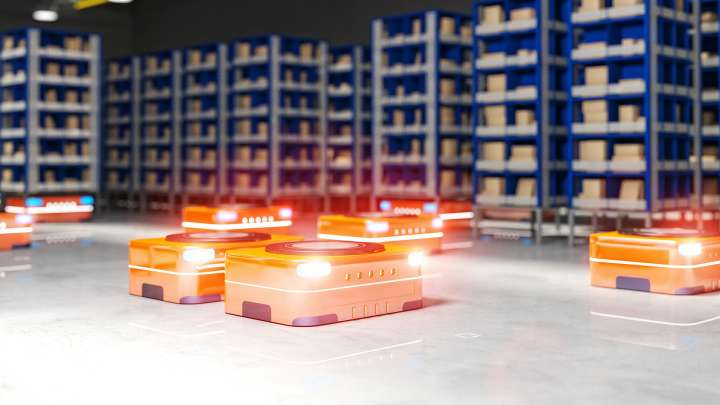
\includegraphics[width=\linewidth]{figures/presentation_specific/amr_warehouse_intel.jpg}
                \caption{AMRs in warehouse \cite{Intel2023}}
                \label{fig:amrs_in_warehouse}
            \end{figure}
        \end{column}%
    \end{columns}%
    \note<1>[item]{These days, there are a lot of different modules that are running on autonomous mobile robots. In order for them to function independently, they would first require a perception module to detect and understand their environment. As you can see, the ARMs are usually equipped with different sensors. Then, the robot needs to know its own location and if there’s no map information, the robot also needs to generate a map. That’s why it needs a SLAM module. Also, to go from point A to point B, the robot needs navigation and a path-planning module. The AMRs also need a control module that controls the actuators.}
    \note<2>[item]{ With all these modules running on the robot, the robot requires a great number of computation resources, but the onboard system that comes with the robot is usually very limited for a couple of reasons. First, there’s the cost of such a big system that can provide computation capabilities. Also, the space and the energy on the robot are also limited. That’s why it’s hard for the robot’s onboard system to run all those modules locally. }
\end{frame}

\begin{frame}{Task Offloading}
    \begin{figure}
        \centering
        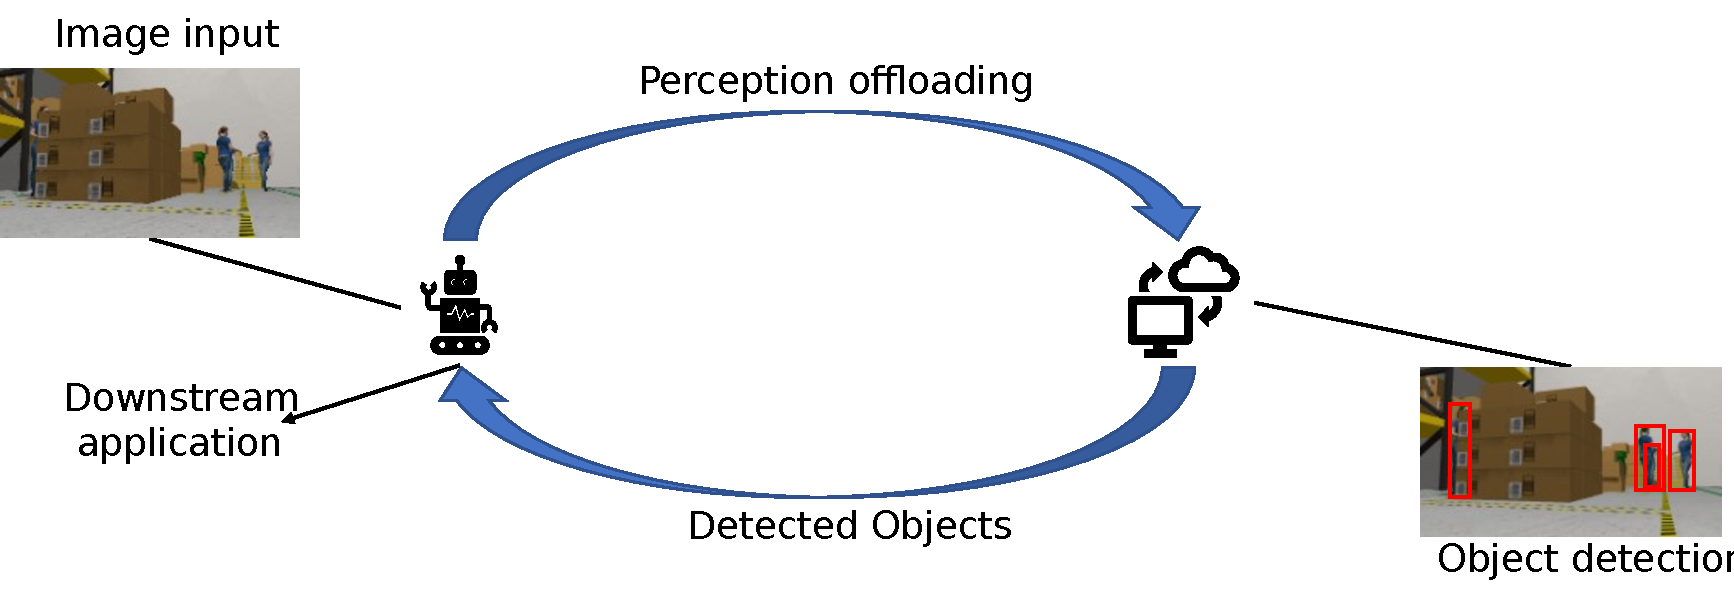
\includegraphics[width=\linewidth]{figures/presentation_specific/task_offloading.pdf}
        \caption{Robotic computation offloading}
        \label{fig:task_offloading}
    \end{figure}
\end{frame}
\note{
This is the issue that the task offloading is trying to tackle. The idea is that instead of running everything on a very limited system onboard, the robot offloads some of the computation tasks, such as object detection via network to the cloud which has abundant resources. Then, the cloud does the computation and sends the processed results back to the robot. From then, the results can be used for some downstream applications, such as navigation and obstacle avoidance.
}

\begin{frame}{Problems}
    \begin{itemize}
        \item<1-> Why offloading tasks?
        \begin{itemize}
            \item Reduce onboard resource usage
            \item Improve task performance
        \end{itemize}
        \item<2-> Current problems with task offloading
        \begin{itemize}
            \item Safety issues -> local computation
            \item Real-time execution -> edge computing
        \end{itemize}
        \item<3-> When and how to offload?
        \begin{itemize}
            \item Dynamic network conditions
            \item Onboard resources
        \end{itemize}
    \end{itemize}
    \note<1>[item]{Offloading all these computation tasks can reduce onboard resource usage. Also, with the more powerful computation capabilities of the cloud, task performance can be greatly improved. Take robot perception as an example. We can only fit a small object detection model on the robot, but we have a rather complex model on the cloud and it will produce more precise detection.}
    \note<2>[item]{However, there are several issues with the computation offloading. First, the network connection may not be stable, so the robot can lose the total connection and cannot process the tasks anymore. To deal with this, the robot needs a local computation on its onboard system that can continue to compute the task even if it’s no longer connected. On the other hand, even if the robot can get the processed results back from the cloud, it might take a really long time. A lot of these tasks running on the robot are also time-sensitive. This is essentially what edge computing is trying to address. The idea of edge computing is to compute the data at the edge of the network, near the robots. For example, this could be a computer located near the robot. This could help reduce the latency of going over multiple hops to reach the cloud.}
    \note<3>[item]{With the options either to compute locally or to offload to the edge computer, another question arises. When should the computation be offloaded? There are many criteria for that. For example, under a bad network connection, it makes more sense for the robot to compute it locally, because it would guarantee that it will generate some results, so the dynamic changes in the network connection are important for the robot to get a good result from computation offloading. Or for example, if the robot has already different tasks running and the CPU usage is high, then you may not want to compute your tasks there because it would slow down other tasks as well. This is the problem I wanted to investigate with my thesis.}
\end{frame}

% ############
% related work
% ############

\begin{frame}{Related Work}
    \begin{itemize}
        \item<1-> Mathematical optimization approaches
        \begin{itemize}
            \item Formulates an optimization problem with a computational model
            \item Minimizes execution latency and/or energy consumption
        \end{itemize}
        \item<2-> Game-theory approaches
        \begin{itemize}
            \item Formulate the problem as a game
        \end{itemize}
        \item<3-> Deep reinforcement learning approaches
        \begin{itemize}
            \item Uses deep RL agent to make offloading decisions -> high inference time
        \end{itemize}
    \end{itemize}
    % notes
    \note<1>[item]{There have been some works in this area already. To start with, some works approach this problem as a pure mathematical optimization problem. They formulate the problem based on a computational model and define an optimization goal. Usually, they are trying to reduce the latency and/or power consumption. The offloading strategy is retrieved from the optimum or sub-optimum of the problem.}
    \note<2>[item]{There are other approaches trying to formulate the optimization problem as a game and using game theory to find an offloading strategy. These methods are very capable of handling the offloading problem of multiple agents and edge computers, but they are all using a computational model, which is constantly changing in a dynamic network condition.}
    \note<3>[item]{Some approaches have taken the dynamic changes into consideration. For example, some approaches train a Deep Reinforcement Learning agent to make the offloading decision based on the runtime parameters of the offloading system. They are showing indeed an improvement in handling the fluctuation in network conditions, but the inference time of the deep neural network used by the reinforcement learning agent would add more latency to the decision-making process and the entire task execution. This is undesired for time-sensitive tasks like object detection and navigation. Therefore, I wanted to find out how the offloading strategies are affecting task performance and resource usage and develop another dynamic offloading strategy that can adapt to dynamic network changes and achieve real-time execution.}
\end{frame}

\begin{frame}{Robot Perception Offloading}
    \begin{figure}
        \centering
        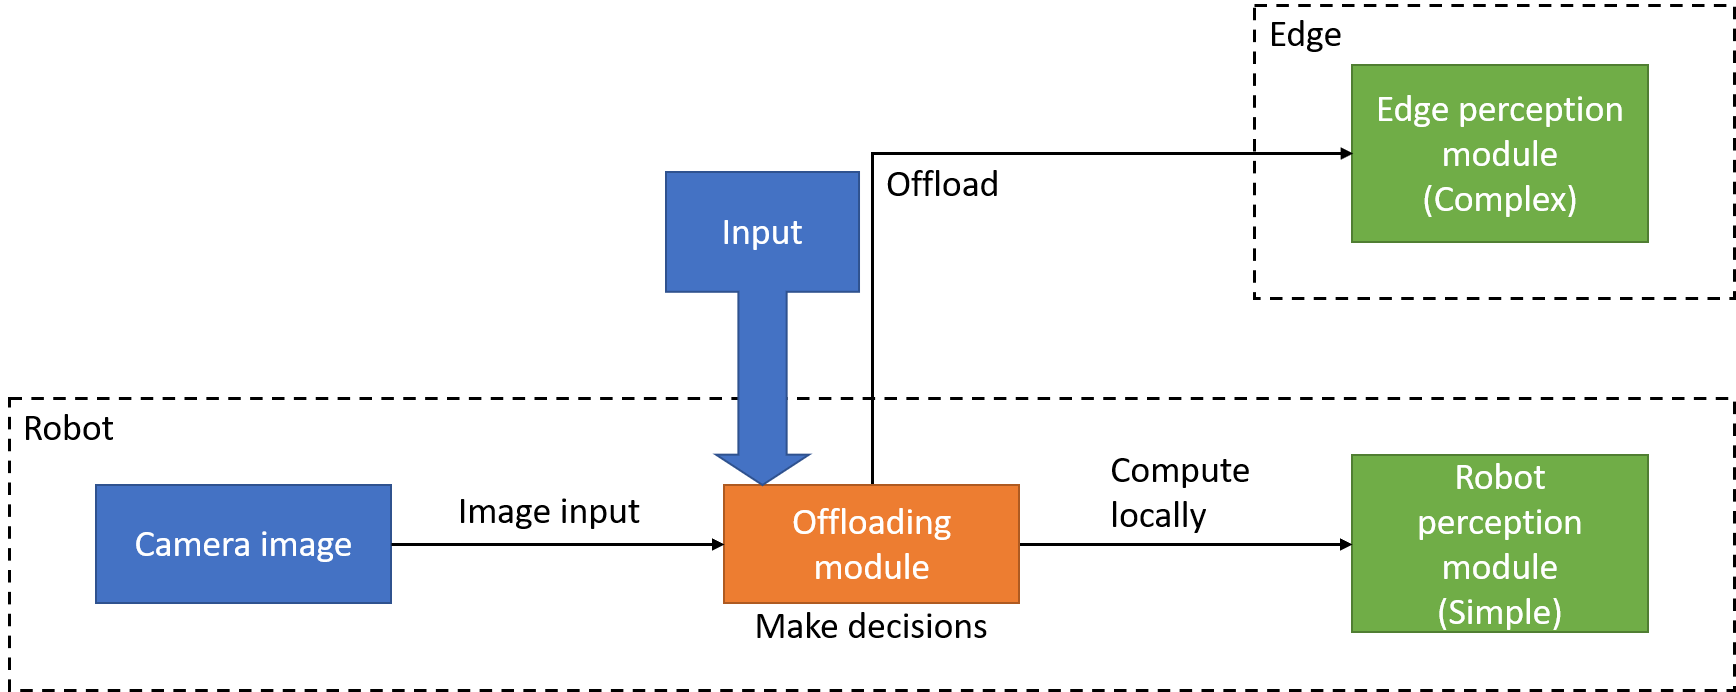
\includegraphics[width=0.8\linewidth]{figures/presentation_specific/robot_perception_offloading.png}
        \caption{Robot perception offloading}
        \label{fig:robot_perception_offloading}
    \end{figure}
\end{frame}
\note{
To investigate this problem, I used object detection as an example for the computation task and designed an offloading pipeline for the robot perception offloading. First, you would have an image coming from the camera sensor and it will be input into the offloading module. The offloading module then makes the decision based on some input from the system, which could be the status of the onboard resources and the network conditions. Then, the offloading module makes the decision of whether to use the local computation module, which usually uses some simple object detection model onboard. Or it can decide to offload to the edge via the network and uses the more complex model on the edge.
}

\begin{frame}{Offloading Framework}
    \begin{figure}
        \centering
        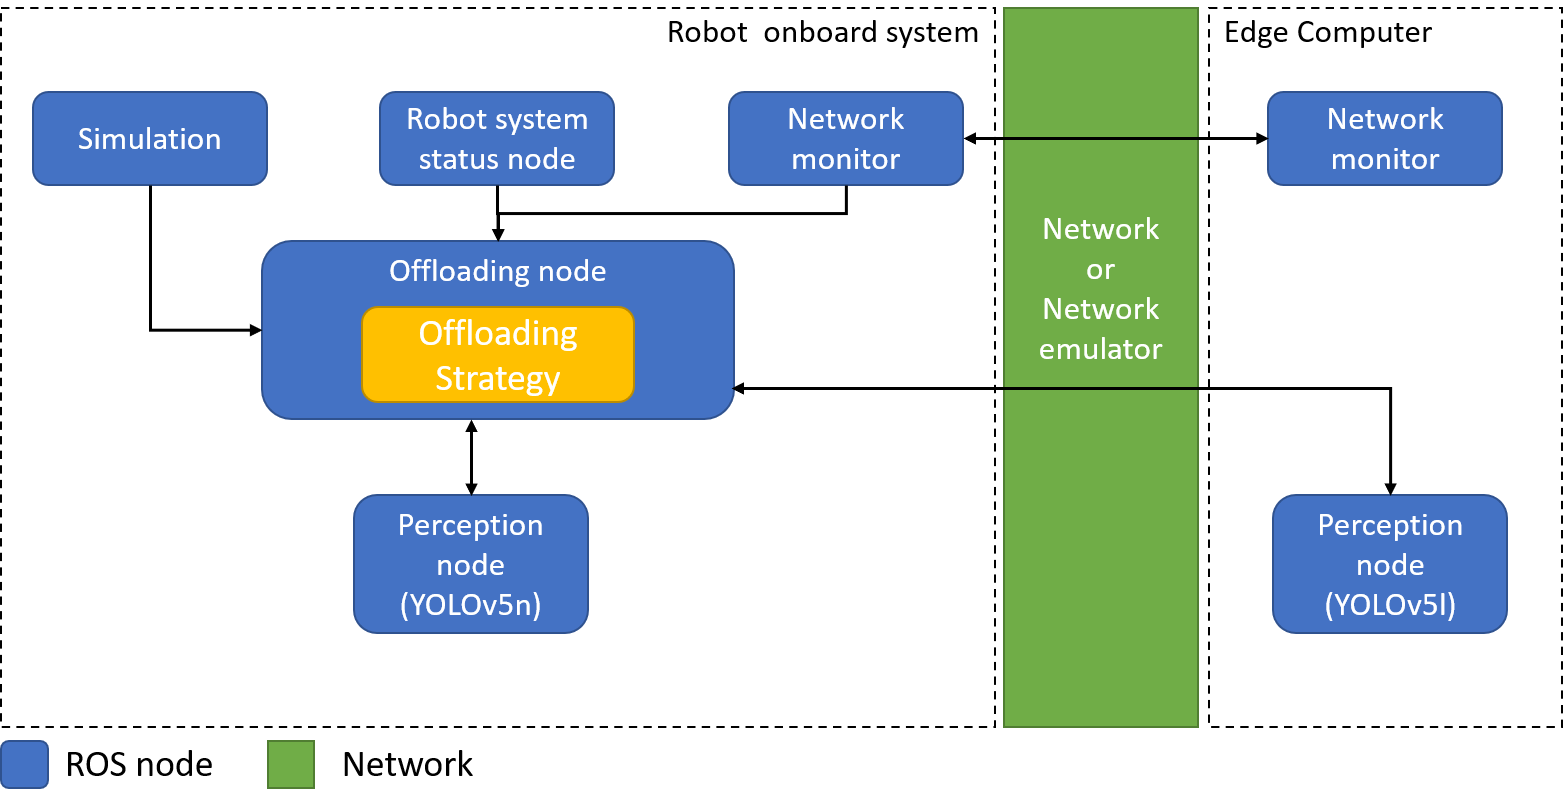
\includegraphics[width=0.7\linewidth]{figures/presentation_specific/offloading_framework.png}
        \label{fig:offloading_framework}
    \end{figure}
\end{frame}
\note{
To realize perception offloading, I implemented an offloading framework using ROS2. The reason that I chose ROS2 as the middleware for the implementation is that first, it has different communication patterns and it allows multi-casting, which would make the deployment of different modules on different machines easier and more reliable. For object detection algorithms, I used the pre-trained YOLOv5 models, because it offers a series of object detection models of different sizes. On the robot, lightweight object detection like the YOLOv5n is deployed. For the edge computer, I use a bigger model, the YOLOv5l. The robot and the edge are connected via a network. There are also different nodes that are monitoring the status of the robot system and the network condition. They pass the information to the offloading node for decision-making. 
}

\begin{frame}{Baseline Strategies}
    \begin{figure}
        \centering
        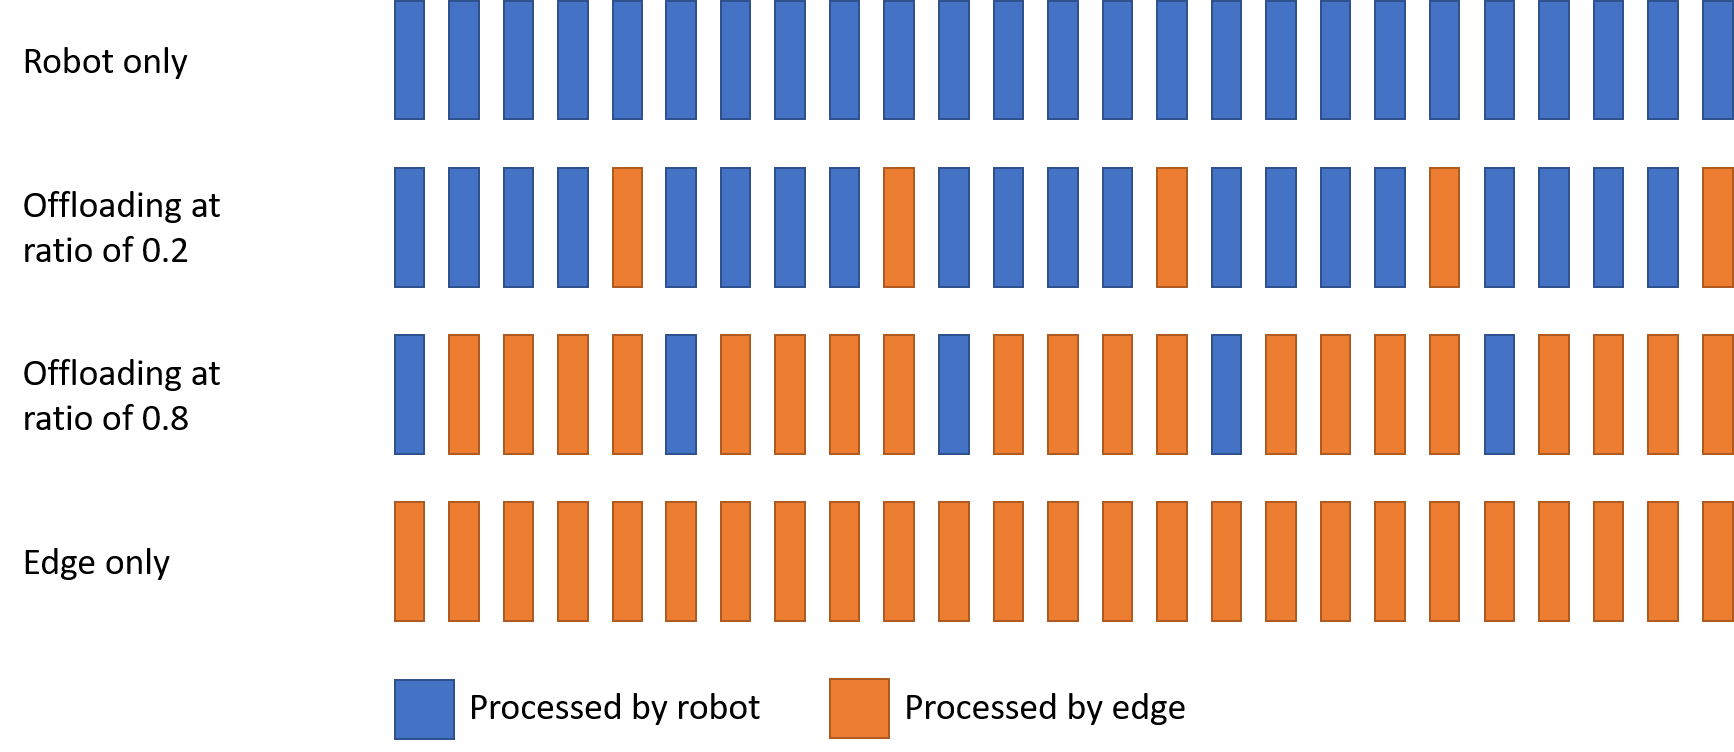
\includegraphics[width=0.8\linewidth]{figures/presentation_specific/baseline_strategies.png}
    \end{figure}
\end{frame}
\note{
To find out how the systems are behaving, I first used some naïve baseline strategies. The “robot only” strategy only computes locally and does not use the edge computer at all. Also, I implemented a ratio strategy that can offload at a given ratio. For example, if the offloading ratio is set to 0.2, the offloading module would offload once every five images. If the ratio is set to 0.8, the offloading module would offload four out of five images to the edge and only compute one image locally. In the end, there’s also the “edge only” strategy that only offloads to the edge and doesn’t use the onboard system. 
}

\begin{frame}{Simulated Scenario}
    \begin{columns}[T,onlytextwidth]%
        \begin{column}[T]{0.48\textwidth}%
            \begin{itemize}
                \item<1-> Environment
                \begin{itemize}
                    \item Industrial warehouse
                    \item Human and other obstacles
                    % \item Recorded as ROS bag and replayed during the experiment
                \end{itemize}
                \item<2-> Robot
                \begin{itemize}
                    \item Equipped with RGB camera
                    \item Navigation through the scene
                \end{itemize}
            \end{itemize}
        \end{column}%
        \begin{column}[T]{0.48\textwidth}%
            \begin{figure}
                \centering
                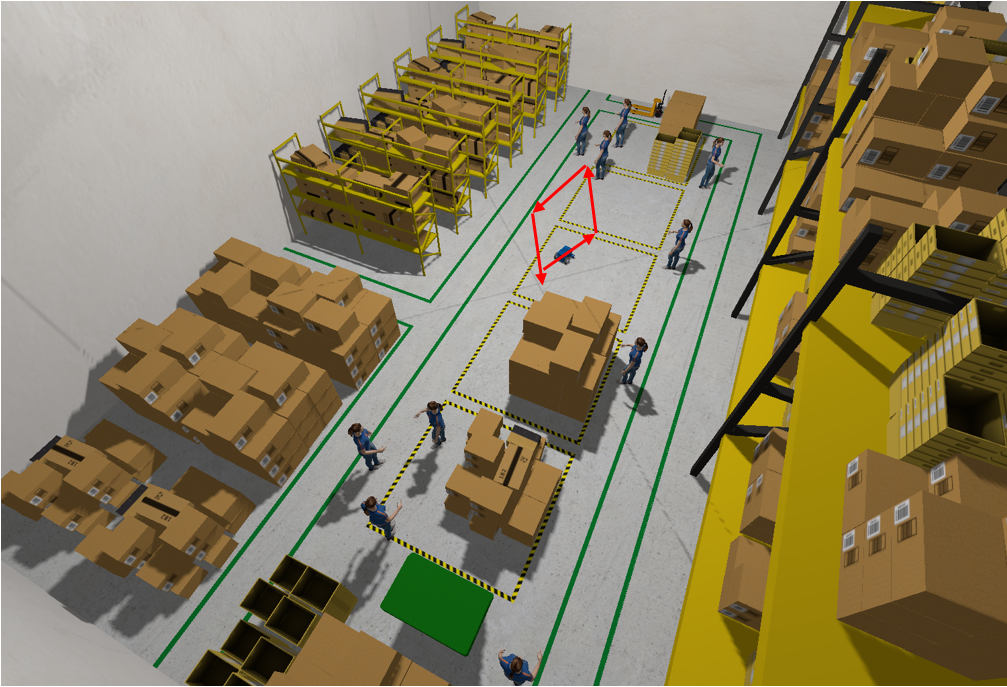
\includegraphics[width=\linewidth]{figures/presentation_specific/bird_view_drawn.png}
                \caption{Simulated scenario}
                \label{fig:simulated_scenario}
            \end{figure}
        \end{column}%
    \end{columns}%
    \note<1>[item]{To test these offloading strategies, I implemented a simulated scenario in Gazebo that simulates a warehouse environment, which is a quite common use case for autonomous mobile robots.  In the environment, I introduced both humans and other objects are obstacles.}
    \note<2>[item]{A robot equipped with an RGB camera is navigating itself through the scene. The red line is the route of the AMR. The RGB camera on top of the robot outputs an image stream of 30 FPS. The image stream is used as the input of the offloading framework}
\end{frame}

\begin{frame}{Metrics}
    \begin{itemize}
        \item<1-> Task performance
        \begin{itemize}
            \item Average precision
            \item Overall processed frames
            \item Perception round-trip time
        \end{itemize}
        \item<2-> Resource usage
        \begin{itemize}
            \item CPU usage
            \item CPU power consumption
            \item Bandwidth usage
        \end{itemize}
    \end{itemize}
    \note<1>[item]{In order to be able to compare different offloading strategies and assess how well they perform. I chose several metrics. They mainly fall into two categories. The first category measures how well the object detection task is performed. This includes the average precision, which measures the precision of the bounding box detection, the overall processed frames, which measures how many frames are eventually processed by either perception module, and the round-trip time measures the time of one image going from the offloading module to the perception module and back, which represents the execution latency.}
    \note<2>[item]{On the other hand, the second category includes the metrics of the AMR’s onboard resource usage. This includes CPU usage and power consumption. If the network is considered as a type of resource, which in case it should be, bandwidth usage measures how much of the network as a type of resource is used.}
\end{frame}

% \begin{frame}{Experimental Setup}
%     \begin{itemize}
%         \item<1-> Simulation
%         \begin{itemize}
%             \item Use Docker containers as virtualization of robot and edge systems
%             \item Use Docker bridge as the virtual network interface
%         \end{itemize}
%         \item<2-> Robot experiment
%         \begin{itemize}
%             \item Robot: Intel NUC with an i3 CPU and no GPUs
%             \item Edge: equipped with an i9 CPU and a GPU
%             \item Network: Ethernet w/wo bandwidth constraints, Wi-Fi
%         \end{itemize}
%     \end{itemize}
%     \note<1>[item]{With these works in place, I started to conduct experiments. The first thing I did was test how the offloading framework is performing under simulation. I used docker containers as virtualization of the AMR’s onboard system and the edge computer. I used the docker bridge as a virtual network interface between the robot and the edge. I tried to test the functionalities of the offloading framework.}
%     \note<2>[item]{After I determined it was working properly, I moved the experiments to actual systems. For the robot onboard system, I used an Intel NUC device, which is equipped with an i3 CPU but without any GPUs. For the edge computer, I used a workstation with a 10-core i9 CPU. It’s also equipped with an Nvidia GTX1060 GPU for object detection tasks. Between the NUC and the edge computer, I first tested the offloading strategies using Ethernet with constrained and unconstrained bandwidth to see how they performed. After that, I also tested them with a Wi-Fi connection, which is subjected to dynamic changes.}
% \end{frame}

\begin{frame}{Synchronous Evaluation}
    \begin{figure}
        \centering
        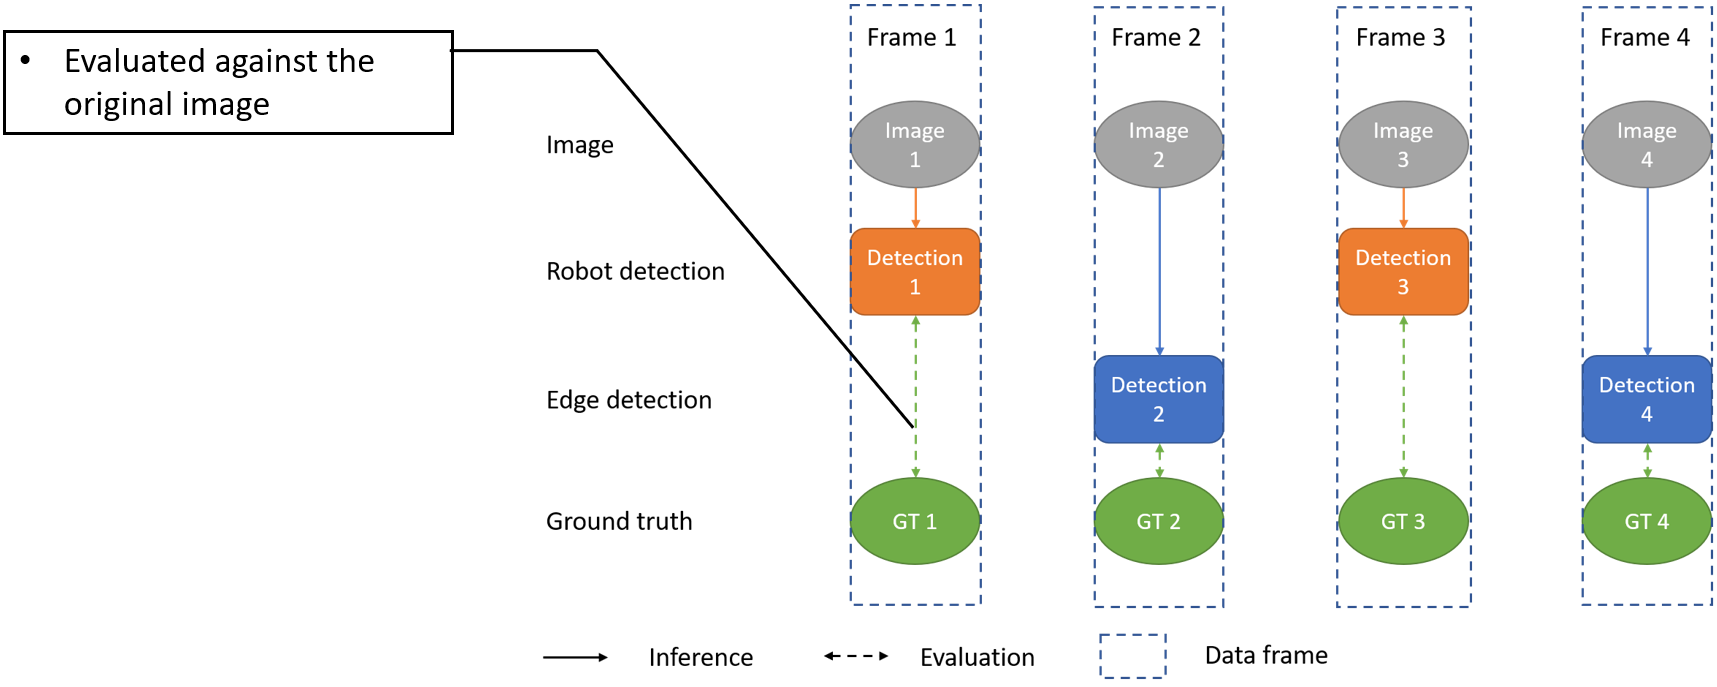
\includegraphics[width=0.8\linewidth]{figures/presentation_specific/sync_eval_annotated.png}
        \label{fig:sync_eval}
    \end{figure}
\end{frame}
\note{When evaluating the data based on the defined metrics, I actually ran into a bit of an issue with the average precision. Initially, I used this synchronous evaluation method. How it works is that the detection generated by the robot or edge perception node is compared against the bounding box ground truth. This means the detection is always compared with the ground truth corresponding to the original image, but this is hardly the case in the real world, because these object detection tasks usually take quite some time to process and to be transmitted back and forth via the network, which means during that time, the robot can already be in a different position. This is more prominent when the robot is rotating, the objects change drastically between frames.}

\begin{frame}{Asynchronous Evaluation}
    \begin{figure}
        \centering
        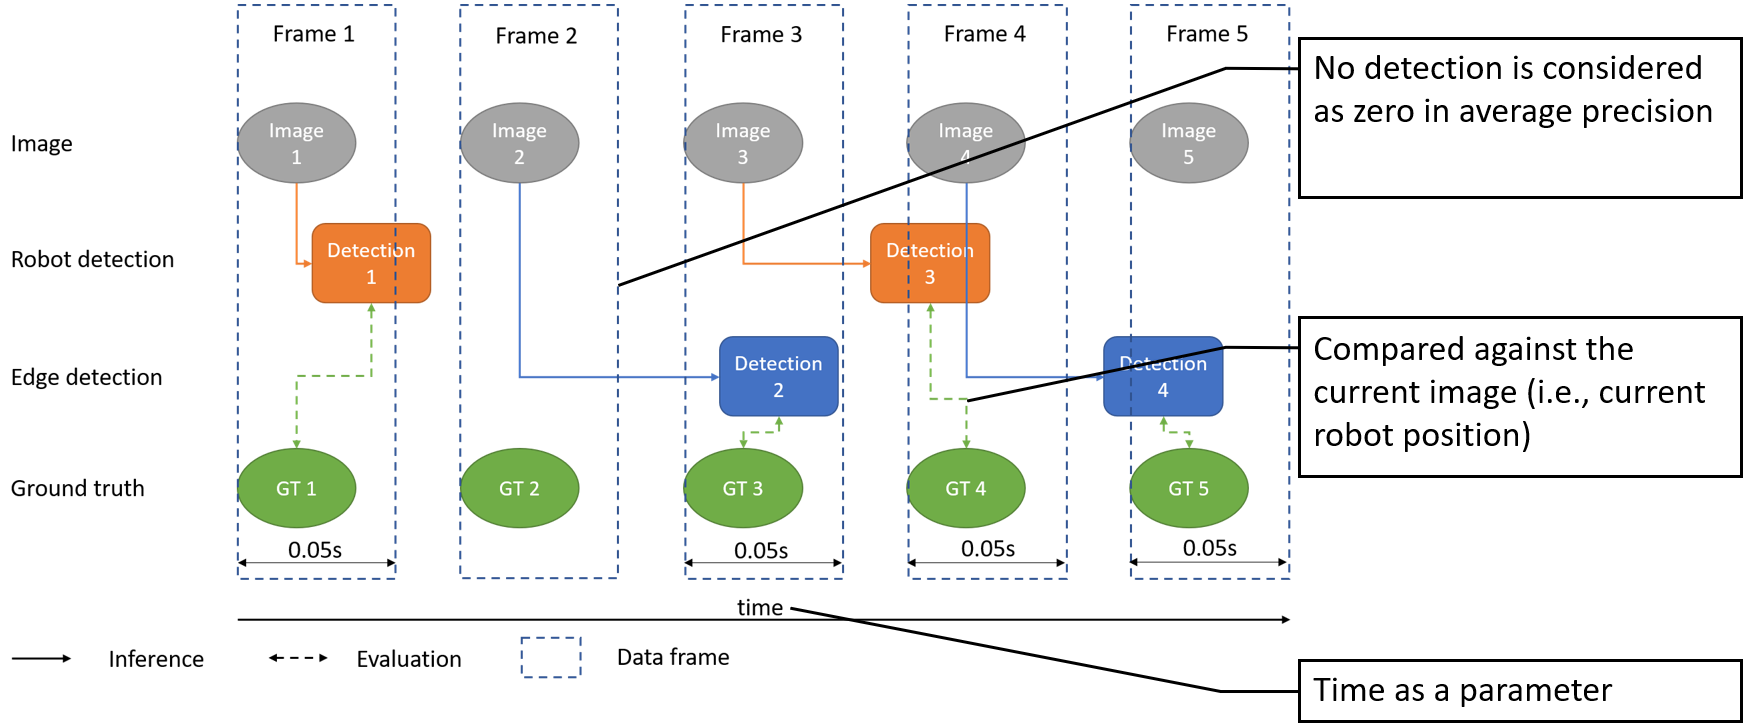
\includegraphics[width=0.8\linewidth]{figures/presentation_specific/async_eval_annotated.png}
        \label{fig:async_eval}
    \end{figure}
\end{frame}
\note{To deal with that problem, I eventually moved on to use an asynchronous evaluation method. The basic idea is that we consider each image as a frame that extends to a certain period of time. Within the period, if the robot receives detection, the detection will be evaluated with the current ground truth data. This method introduces time as a parameter and takes the execution latency into consideration of the average precision. Under this evaluation method, if a frame can't be matched with any detection, it means that the robot has no information about its environment during that time and it would be considered zero in the average precision.}

% ################################
% Results from baseline strategies
% ################################
\begin{frame}{Results of Baseline Strategies}
    \begin{figure}
        \centering
        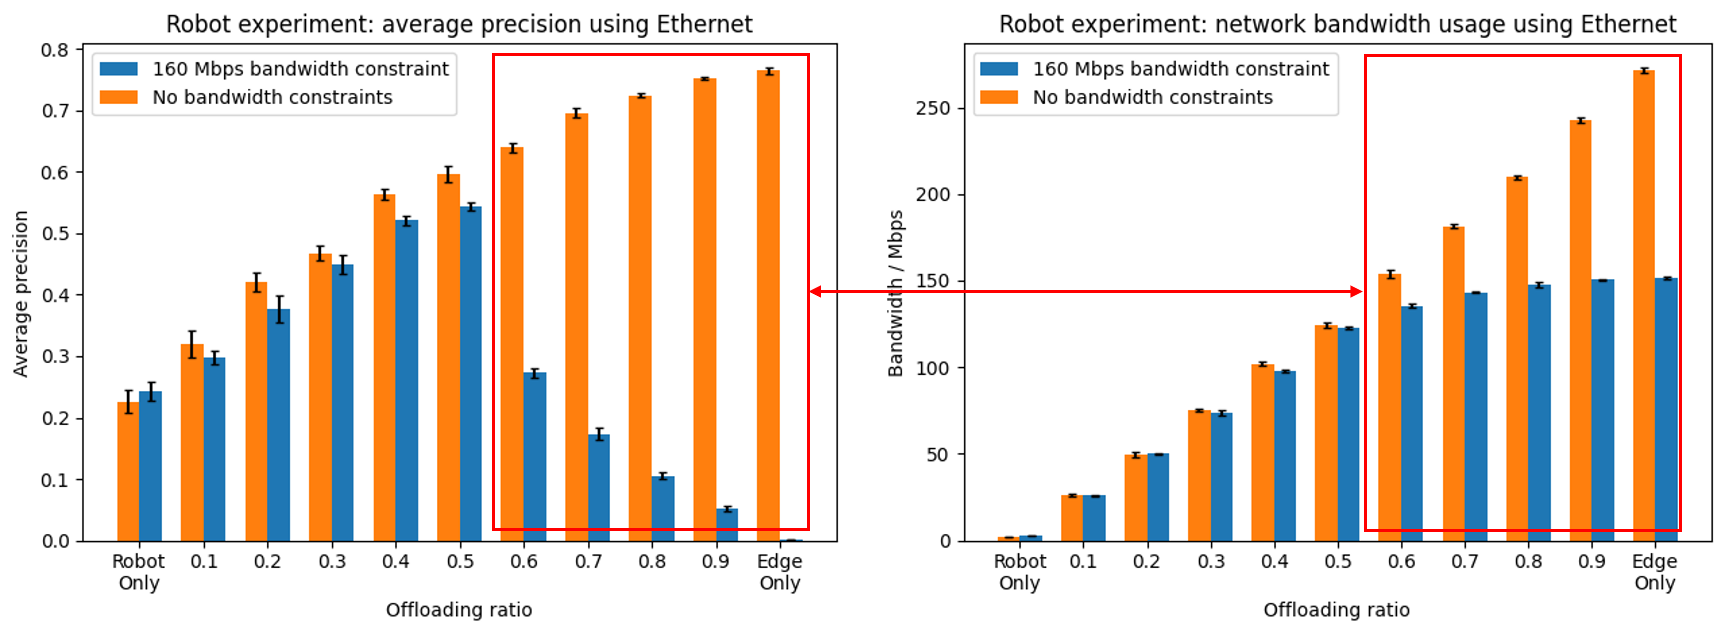
\includegraphics[width=\linewidth]{figures/presentation_specific/baseline_results_1.png}
    \end{figure}
\end{frame}
\note{First, I tested the baseline strategies using the Ethernet w/wo additional bandwidth constraints. The left-hand side image shows the average precision of different offloading strategies tested with Ethernet. The right-hand side image shows the network bandwidth usage. The x-axis is the offloading ratio, increasing from “robot only” to “edge only”. From the results, we can see that if the network bandwidth is constrained, the average precision will drop when the band is saturated, but if the network bandwidth is unconstrained, the average precision will continue to improve with more frames calculated by the edge. This is caused by two reasons. First, the edge computer has a more complex object detection module that can produce more precise detection. Second, the edge computer is able to compute the inference more quickly and thus computes more frames. This also causes the overall average precision to improve.}

% \begin{frame}{Results of Baseline Strategies}
%     \begin{figure}
%         \centering
%         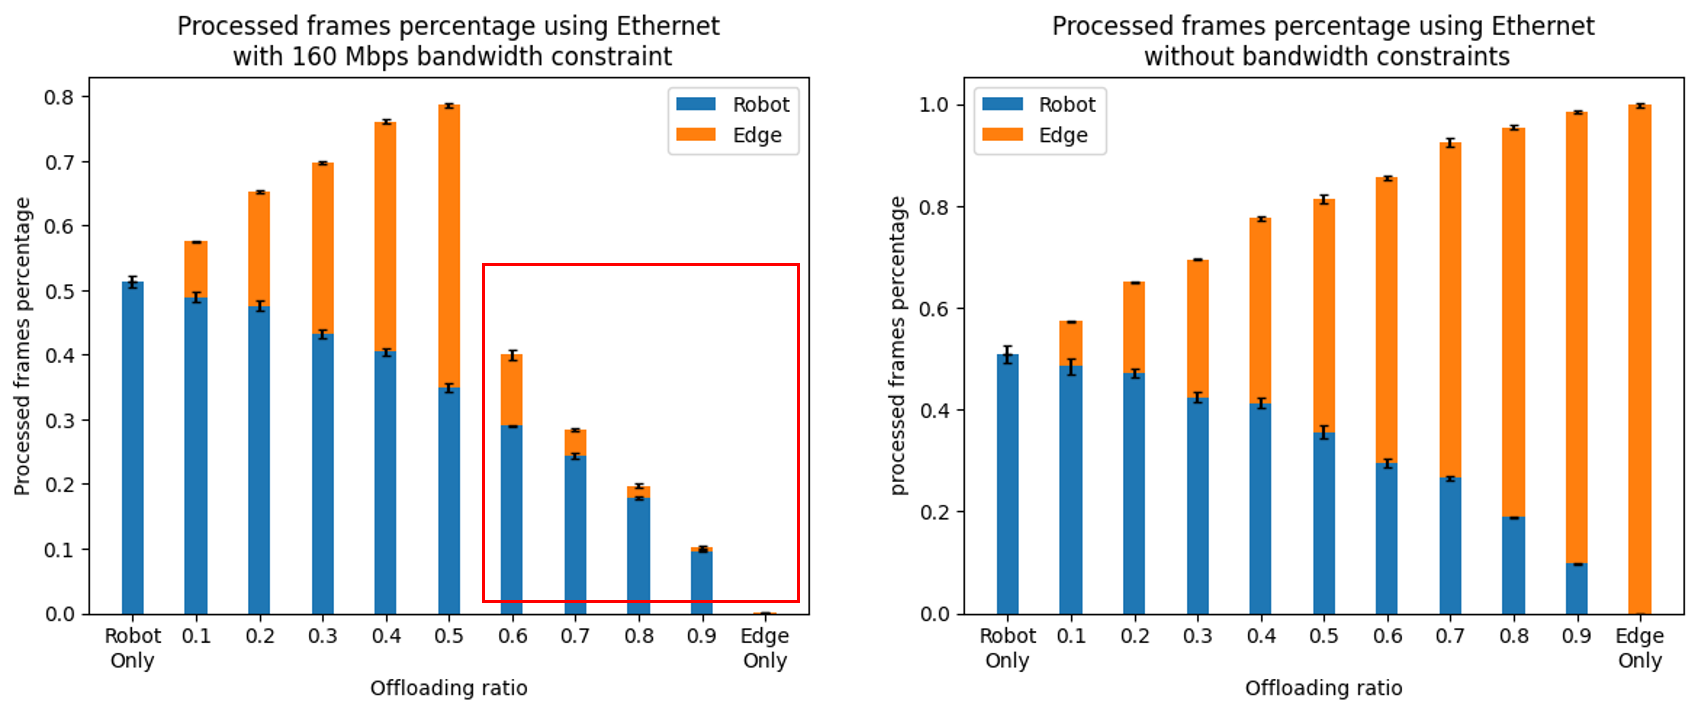
\includegraphics[width=0.9\linewidth]{figures/presentation_specific/baseline_results_2.png}
%     \end{figure}
% \end{frame}
% \note{Second, when the network is not constrained, the edge computer can compute more image frames and causes the average precision to increase. In this slide, the left image shows how many images are processed when the network is constrained and the right image shows the unconstrained version. This part corresponds to the bandwidth saturation in the last slide. }

\begin{frame}{Results of Baseline Strategies}
    \begin{figure}
        \centering
        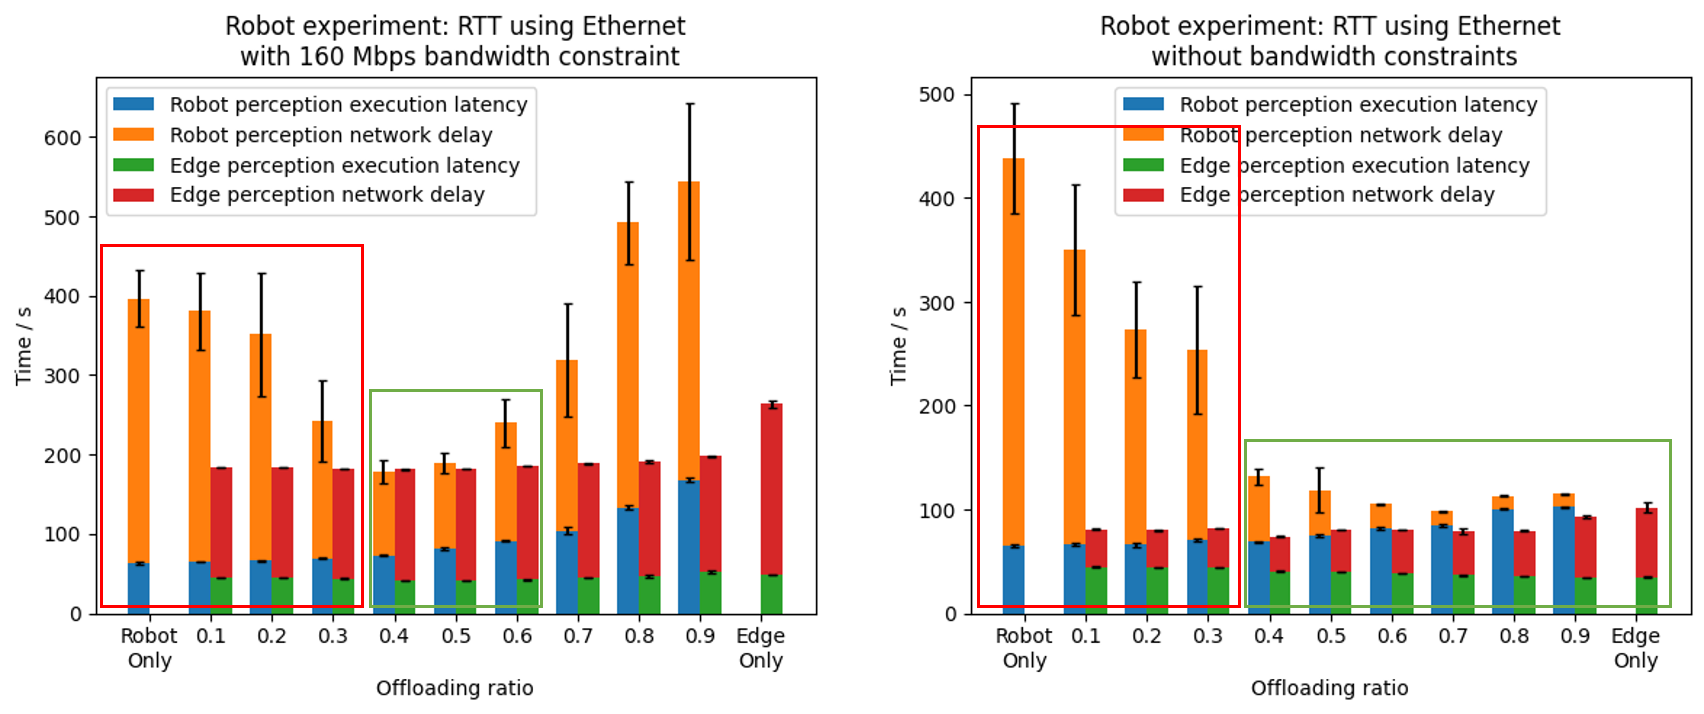
\includegraphics[width=0.9\linewidth]{figures/presentation_specific/baseline_results_3.png}
    \end{figure}
\end{frame}
\note{ In terms of the round-trip time, the robot perception module is not able to handle all the frames on its onboard system, so the latency of the robot perception increases when more frames are processed on the robot. The frames start to queue and wait to be processed. If the network is constrained, there’s also a local minimum that occurs around the 0.4 to 0.6 offloading ratio. At this stage, the onboard perception module is no longer strained and the network bandwidth is not saturated. After the bandwidth saturation, the execution delay increases. However, this is not seen for the unconstrained network. This shows that the round-trip time can reflect the available network bandwidth and onboard resources.}

% \begin{frame}{Results of Baseline Strategies}
%     \begin{figure}
%         \centering
%         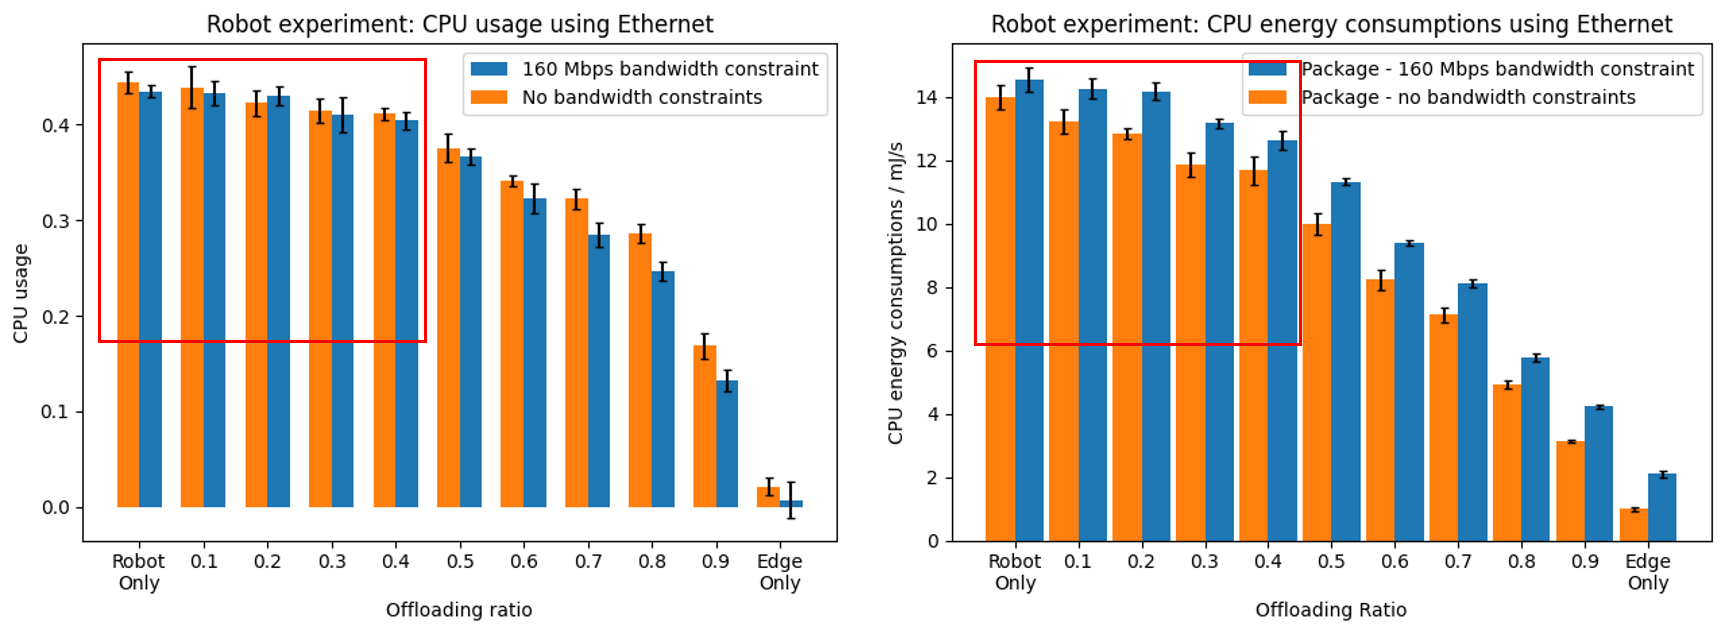
\includegraphics[width=\linewidth]{figures/presentation_specific/baseline_results_4.png}
%     \end{figure}
% \end{frame}

\begin{frame}{Results of Baseline Strategies}
    \begin{itemize}
        \item<1-> Network bandwidth is the main constraint of edge task performance -> hard to measure during runtime
        \item<2-> Round-trip time as an indicator for network conditions and onboard computation resources
        \item<3-> Balance between network resources and computation resources
    \end{itemize}
    \note<1>[item]{From the results of the baseline strategies, we can tell that the network bandwidth is clearly a constrain for the task performance of the edge computer, but the available bandwidth is hard to measure during runtime because you have to pause your tasks and send bytes back and forth for an extended period of time.}
    \note<2>[item]{The solution that I propose is that we can use round-trip time, which can be measured more easily during runtime, as an indicator for network conditions and onboard computation resources. Based on the round-trip time, we can make sure that the perception node is not overwhelmed or the bandwidth is not saturated.}
    \note<3>[item]{In general, the offloading strategies should balance between the available network resources and the onboard computation resources.}
\end{frame}

% ################
% Dynamic strategy
% ################

\begin{frame}{Dynamic Offloading Strategy}
    \begin{figure}
        \centering
        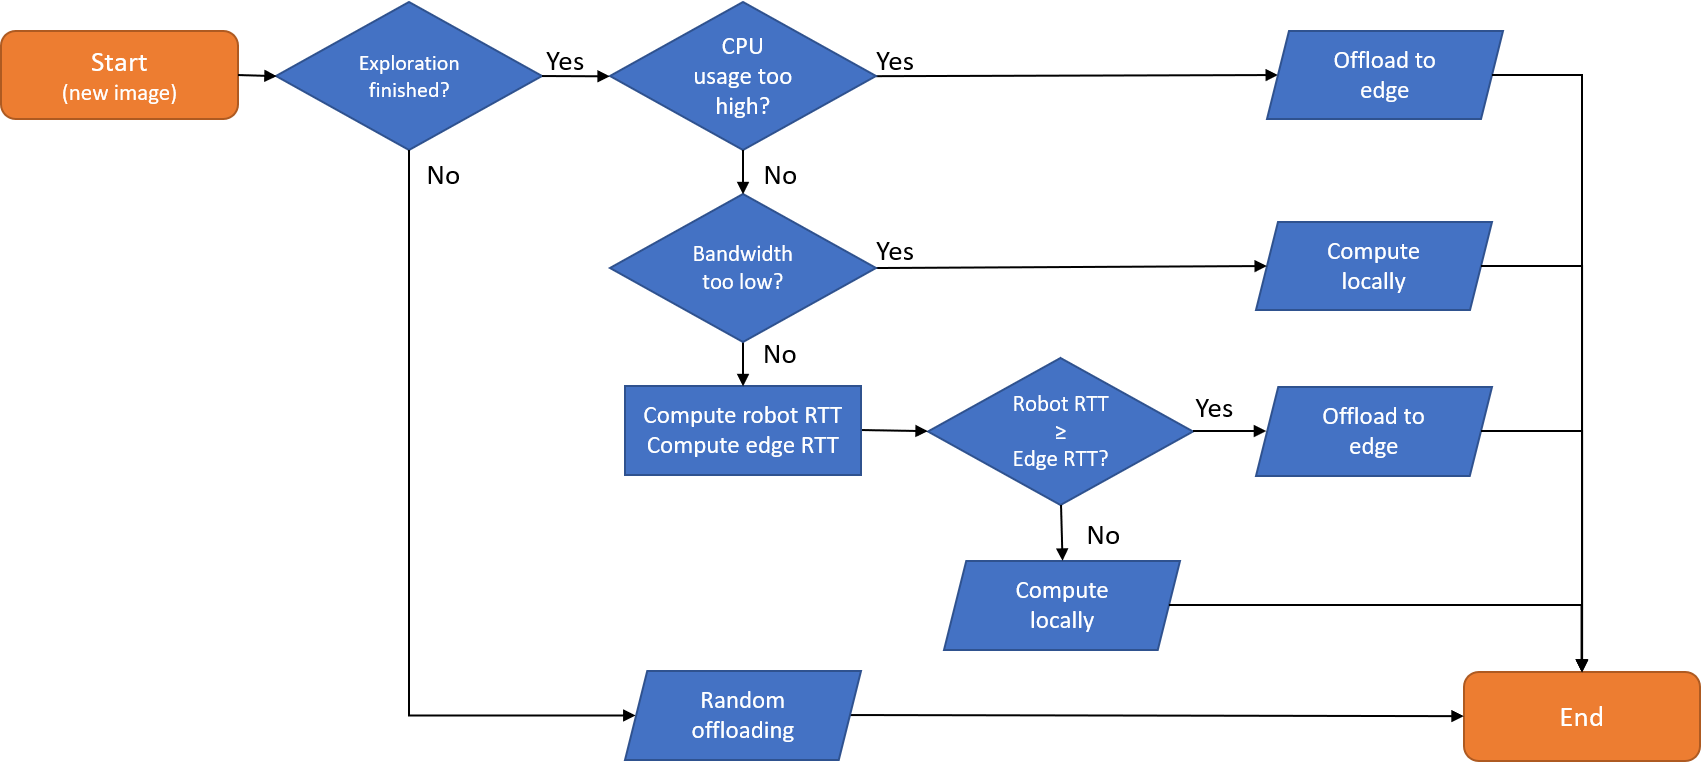
\includegraphics[width=0.8\linewidth]{figures/presentation_specific/dynamic_offloading_strategy.png}
    \end{figure}
\end{frame}
\note{Using round-trip time as an indicator, I developed and implemented a dynamic offloading strategy. At start-up, the dynamic offloading strategy would go through an exploration stage, where it makes random offloading decisions to get the first measurement of the system states. After the exploration stage, the offloading strategy would in turn check for CPU usage and bandwidth usage. If they exceed certain limits, the dynamic offloading strategy would choose to offload or to compute locally respectively. After that, it would use the round-trip time of the edge perception and the robot perception as an indicator and chooses the perception module that has the lowest round-trip time to process.}

\begin{frame}{Results of Dynamic Offloading Strategy}
    \begin{figure}
        \centering
        \scalebox{0.75}{%% Creator: Matplotlib, PGF backend
%%
%% To include the figure in your LaTeX document, write
%%   \input{<filename>.pgf}
%%
%% Make sure the required packages are loaded in your preamble
%%   \usepackage{pgf}
%%
%% Also ensure that all the required font packages are loaded; for instance,
%% the lmodern package is sometimes necessary when using math font.
%%   \usepackage{lmodern}
%%
%% Figures using additional raster images can only be included by \input if
%% they are in the same directory as the main LaTeX file. For loading figures
%% from other directories you can use the `import` package
%%   \usepackage{import}
%%
%% and then include the figures with
%%   \import{<path to file>}{<filename>.pgf}
%%
%% Matplotlib used the following preamble
%%   
%%   \makeatletter\@ifpackageloaded{underscore}{}{\usepackage[strings]{underscore}}\makeatother
%%
\begingroup%
\makeatletter%
\begin{pgfpicture}%
\pgfpathrectangle{\pgfpointorigin}{\pgfqpoint{6.400000in}{4.800000in}}%
\pgfusepath{use as bounding box, clip}%
\begin{pgfscope}%
\pgfsetbuttcap%
\pgfsetmiterjoin%
\definecolor{currentfill}{rgb}{1.000000,1.000000,1.000000}%
\pgfsetfillcolor{currentfill}%
\pgfsetlinewidth{0.000000pt}%
\definecolor{currentstroke}{rgb}{1.000000,1.000000,1.000000}%
\pgfsetstrokecolor{currentstroke}%
\pgfsetdash{}{0pt}%
\pgfpathmoveto{\pgfqpoint{0.000000in}{0.000000in}}%
\pgfpathlineto{\pgfqpoint{6.400000in}{0.000000in}}%
\pgfpathlineto{\pgfqpoint{6.400000in}{4.800000in}}%
\pgfpathlineto{\pgfqpoint{0.000000in}{4.800000in}}%
\pgfpathlineto{\pgfqpoint{0.000000in}{0.000000in}}%
\pgfpathclose%
\pgfusepath{fill}%
\end{pgfscope}%
\begin{pgfscope}%
\pgfsetbuttcap%
\pgfsetmiterjoin%
\definecolor{currentfill}{rgb}{1.000000,1.000000,1.000000}%
\pgfsetfillcolor{currentfill}%
\pgfsetlinewidth{0.000000pt}%
\definecolor{currentstroke}{rgb}{0.000000,0.000000,0.000000}%
\pgfsetstrokecolor{currentstroke}%
\pgfsetstrokeopacity{0.000000}%
\pgfsetdash{}{0pt}%
\pgfpathmoveto{\pgfqpoint{0.603704in}{0.549691in}}%
\pgfpathlineto{\pgfqpoint{6.250000in}{0.549691in}}%
\pgfpathlineto{\pgfqpoint{6.250000in}{4.450926in}}%
\pgfpathlineto{\pgfqpoint{0.603704in}{4.450926in}}%
\pgfpathlineto{\pgfqpoint{0.603704in}{0.549691in}}%
\pgfpathclose%
\pgfusepath{fill}%
\end{pgfscope}%
\begin{pgfscope}%
\pgfsetbuttcap%
\pgfsetroundjoin%
\definecolor{currentfill}{rgb}{0.000000,0.000000,0.000000}%
\pgfsetfillcolor{currentfill}%
\pgfsetlinewidth{0.803000pt}%
\definecolor{currentstroke}{rgb}{0.000000,0.000000,0.000000}%
\pgfsetstrokecolor{currentstroke}%
\pgfsetdash{}{0pt}%
\pgfsys@defobject{currentmarker}{\pgfqpoint{0.000000in}{-0.048611in}}{\pgfqpoint{0.000000in}{0.000000in}}{%
\pgfpathmoveto{\pgfqpoint{0.000000in}{0.000000in}}%
\pgfpathlineto{\pgfqpoint{0.000000in}{-0.048611in}}%
\pgfusepath{stroke,fill}%
}%
\begin{pgfscope}%
\pgfsys@transformshift{0.860354in}{0.549691in}%
\pgfsys@useobject{currentmarker}{}%
\end{pgfscope}%
\end{pgfscope}%
\begin{pgfscope}%
\definecolor{textcolor}{rgb}{0.000000,0.000000,0.000000}%
\pgfsetstrokecolor{textcolor}%
\pgfsetfillcolor{textcolor}%
\pgftext[x=0.860354in,y=0.452469in,,top]{\color{textcolor}\rmfamily\fontsize{10.000000}{12.000000}\selectfont \(\displaystyle {0}\)}%
\end{pgfscope}%
\begin{pgfscope}%
\pgfsetbuttcap%
\pgfsetroundjoin%
\definecolor{currentfill}{rgb}{0.000000,0.000000,0.000000}%
\pgfsetfillcolor{currentfill}%
\pgfsetlinewidth{0.803000pt}%
\definecolor{currentstroke}{rgb}{0.000000,0.000000,0.000000}%
\pgfsetstrokecolor{currentstroke}%
\pgfsetdash{}{0pt}%
\pgfsys@defobject{currentmarker}{\pgfqpoint{0.000000in}{-0.048611in}}{\pgfqpoint{0.000000in}{0.000000in}}{%
\pgfpathmoveto{\pgfqpoint{0.000000in}{0.000000in}}%
\pgfpathlineto{\pgfqpoint{0.000000in}{-0.048611in}}%
\pgfusepath{stroke,fill}%
}%
\begin{pgfscope}%
\pgfsys@transformshift{1.886953in}{0.549691in}%
\pgfsys@useobject{currentmarker}{}%
\end{pgfscope}%
\end{pgfscope}%
\begin{pgfscope}%
\definecolor{textcolor}{rgb}{0.000000,0.000000,0.000000}%
\pgfsetstrokecolor{textcolor}%
\pgfsetfillcolor{textcolor}%
\pgftext[x=1.886953in,y=0.452469in,,top]{\color{textcolor}\rmfamily\fontsize{10.000000}{12.000000}\selectfont \(\displaystyle {2}\)}%
\end{pgfscope}%
\begin{pgfscope}%
\pgfsetbuttcap%
\pgfsetroundjoin%
\definecolor{currentfill}{rgb}{0.000000,0.000000,0.000000}%
\pgfsetfillcolor{currentfill}%
\pgfsetlinewidth{0.803000pt}%
\definecolor{currentstroke}{rgb}{0.000000,0.000000,0.000000}%
\pgfsetstrokecolor{currentstroke}%
\pgfsetdash{}{0pt}%
\pgfsys@defobject{currentmarker}{\pgfqpoint{0.000000in}{-0.048611in}}{\pgfqpoint{0.000000in}{0.000000in}}{%
\pgfpathmoveto{\pgfqpoint{0.000000in}{0.000000in}}%
\pgfpathlineto{\pgfqpoint{0.000000in}{-0.048611in}}%
\pgfusepath{stroke,fill}%
}%
\begin{pgfscope}%
\pgfsys@transformshift{2.913552in}{0.549691in}%
\pgfsys@useobject{currentmarker}{}%
\end{pgfscope}%
\end{pgfscope}%
\begin{pgfscope}%
\definecolor{textcolor}{rgb}{0.000000,0.000000,0.000000}%
\pgfsetstrokecolor{textcolor}%
\pgfsetfillcolor{textcolor}%
\pgftext[x=2.913552in,y=0.452469in,,top]{\color{textcolor}\rmfamily\fontsize{10.000000}{12.000000}\selectfont \(\displaystyle {4}\)}%
\end{pgfscope}%
\begin{pgfscope}%
\pgfsetbuttcap%
\pgfsetroundjoin%
\definecolor{currentfill}{rgb}{0.000000,0.000000,0.000000}%
\pgfsetfillcolor{currentfill}%
\pgfsetlinewidth{0.803000pt}%
\definecolor{currentstroke}{rgb}{0.000000,0.000000,0.000000}%
\pgfsetstrokecolor{currentstroke}%
\pgfsetdash{}{0pt}%
\pgfsys@defobject{currentmarker}{\pgfqpoint{0.000000in}{-0.048611in}}{\pgfqpoint{0.000000in}{0.000000in}}{%
\pgfpathmoveto{\pgfqpoint{0.000000in}{0.000000in}}%
\pgfpathlineto{\pgfqpoint{0.000000in}{-0.048611in}}%
\pgfusepath{stroke,fill}%
}%
\begin{pgfscope}%
\pgfsys@transformshift{3.940152in}{0.549691in}%
\pgfsys@useobject{currentmarker}{}%
\end{pgfscope}%
\end{pgfscope}%
\begin{pgfscope}%
\definecolor{textcolor}{rgb}{0.000000,0.000000,0.000000}%
\pgfsetstrokecolor{textcolor}%
\pgfsetfillcolor{textcolor}%
\pgftext[x=3.940152in,y=0.452469in,,top]{\color{textcolor}\rmfamily\fontsize{10.000000}{12.000000}\selectfont \(\displaystyle {6}\)}%
\end{pgfscope}%
\begin{pgfscope}%
\pgfsetbuttcap%
\pgfsetroundjoin%
\definecolor{currentfill}{rgb}{0.000000,0.000000,0.000000}%
\pgfsetfillcolor{currentfill}%
\pgfsetlinewidth{0.803000pt}%
\definecolor{currentstroke}{rgb}{0.000000,0.000000,0.000000}%
\pgfsetstrokecolor{currentstroke}%
\pgfsetdash{}{0pt}%
\pgfsys@defobject{currentmarker}{\pgfqpoint{0.000000in}{-0.048611in}}{\pgfqpoint{0.000000in}{0.000000in}}{%
\pgfpathmoveto{\pgfqpoint{0.000000in}{0.000000in}}%
\pgfpathlineto{\pgfqpoint{0.000000in}{-0.048611in}}%
\pgfusepath{stroke,fill}%
}%
\begin{pgfscope}%
\pgfsys@transformshift{4.966751in}{0.549691in}%
\pgfsys@useobject{currentmarker}{}%
\end{pgfscope}%
\end{pgfscope}%
\begin{pgfscope}%
\definecolor{textcolor}{rgb}{0.000000,0.000000,0.000000}%
\pgfsetstrokecolor{textcolor}%
\pgfsetfillcolor{textcolor}%
\pgftext[x=4.966751in,y=0.452469in,,top]{\color{textcolor}\rmfamily\fontsize{10.000000}{12.000000}\selectfont \(\displaystyle {8}\)}%
\end{pgfscope}%
\begin{pgfscope}%
\pgfsetbuttcap%
\pgfsetroundjoin%
\definecolor{currentfill}{rgb}{0.000000,0.000000,0.000000}%
\pgfsetfillcolor{currentfill}%
\pgfsetlinewidth{0.803000pt}%
\definecolor{currentstroke}{rgb}{0.000000,0.000000,0.000000}%
\pgfsetstrokecolor{currentstroke}%
\pgfsetdash{}{0pt}%
\pgfsys@defobject{currentmarker}{\pgfqpoint{0.000000in}{-0.048611in}}{\pgfqpoint{0.000000in}{0.000000in}}{%
\pgfpathmoveto{\pgfqpoint{0.000000in}{0.000000in}}%
\pgfpathlineto{\pgfqpoint{0.000000in}{-0.048611in}}%
\pgfusepath{stroke,fill}%
}%
\begin{pgfscope}%
\pgfsys@transformshift{5.993350in}{0.549691in}%
\pgfsys@useobject{currentmarker}{}%
\end{pgfscope}%
\end{pgfscope}%
\begin{pgfscope}%
\definecolor{textcolor}{rgb}{0.000000,0.000000,0.000000}%
\pgfsetstrokecolor{textcolor}%
\pgfsetfillcolor{textcolor}%
\pgftext[x=5.993350in,y=0.452469in,,top]{\color{textcolor}\rmfamily\fontsize{10.000000}{12.000000}\selectfont \(\displaystyle {10}\)}%
\end{pgfscope}%
\begin{pgfscope}%
\definecolor{textcolor}{rgb}{0.000000,0.000000,0.000000}%
\pgfsetstrokecolor{textcolor}%
\pgfsetfillcolor{textcolor}%
\pgftext[x=3.426852in,y=0.273457in,,top]{\color{textcolor}\rmfamily\fontsize{10.000000}{12.000000}\selectfont Offloading ratio}%
\end{pgfscope}%
\begin{pgfscope}%
\pgfsetbuttcap%
\pgfsetroundjoin%
\definecolor{currentfill}{rgb}{0.000000,0.000000,0.000000}%
\pgfsetfillcolor{currentfill}%
\pgfsetlinewidth{0.803000pt}%
\definecolor{currentstroke}{rgb}{0.000000,0.000000,0.000000}%
\pgfsetstrokecolor{currentstroke}%
\pgfsetdash{}{0pt}%
\pgfsys@defobject{currentmarker}{\pgfqpoint{-0.048611in}{0.000000in}}{\pgfqpoint{-0.000000in}{0.000000in}}{%
\pgfpathmoveto{\pgfqpoint{-0.000000in}{0.000000in}}%
\pgfpathlineto{\pgfqpoint{-0.048611in}{0.000000in}}%
\pgfusepath{stroke,fill}%
}%
\begin{pgfscope}%
\pgfsys@transformshift{0.603704in}{0.611903in}%
\pgfsys@useobject{currentmarker}{}%
\end{pgfscope}%
\end{pgfscope}%
\begin{pgfscope}%
\definecolor{textcolor}{rgb}{0.000000,0.000000,0.000000}%
\pgfsetstrokecolor{textcolor}%
\pgfsetfillcolor{textcolor}%
\pgftext[x=0.329012in, y=0.563677in, left, base]{\color{textcolor}\rmfamily\fontsize{10.000000}{12.000000}\selectfont \(\displaystyle {0.1}\)}%
\end{pgfscope}%
\begin{pgfscope}%
\pgfsetbuttcap%
\pgfsetroundjoin%
\definecolor{currentfill}{rgb}{0.000000,0.000000,0.000000}%
\pgfsetfillcolor{currentfill}%
\pgfsetlinewidth{0.803000pt}%
\definecolor{currentstroke}{rgb}{0.000000,0.000000,0.000000}%
\pgfsetstrokecolor{currentstroke}%
\pgfsetdash{}{0pt}%
\pgfsys@defobject{currentmarker}{\pgfqpoint{-0.048611in}{0.000000in}}{\pgfqpoint{-0.000000in}{0.000000in}}{%
\pgfpathmoveto{\pgfqpoint{-0.000000in}{0.000000in}}%
\pgfpathlineto{\pgfqpoint{-0.048611in}{0.000000in}}%
\pgfusepath{stroke,fill}%
}%
\begin{pgfscope}%
\pgfsys@transformshift{0.603704in}{1.277126in}%
\pgfsys@useobject{currentmarker}{}%
\end{pgfscope}%
\end{pgfscope}%
\begin{pgfscope}%
\definecolor{textcolor}{rgb}{0.000000,0.000000,0.000000}%
\pgfsetstrokecolor{textcolor}%
\pgfsetfillcolor{textcolor}%
\pgftext[x=0.329012in, y=1.228901in, left, base]{\color{textcolor}\rmfamily\fontsize{10.000000}{12.000000}\selectfont \(\displaystyle {0.2}\)}%
\end{pgfscope}%
\begin{pgfscope}%
\pgfsetbuttcap%
\pgfsetroundjoin%
\definecolor{currentfill}{rgb}{0.000000,0.000000,0.000000}%
\pgfsetfillcolor{currentfill}%
\pgfsetlinewidth{0.803000pt}%
\definecolor{currentstroke}{rgb}{0.000000,0.000000,0.000000}%
\pgfsetstrokecolor{currentstroke}%
\pgfsetdash{}{0pt}%
\pgfsys@defobject{currentmarker}{\pgfqpoint{-0.048611in}{0.000000in}}{\pgfqpoint{-0.000000in}{0.000000in}}{%
\pgfpathmoveto{\pgfqpoint{-0.000000in}{0.000000in}}%
\pgfpathlineto{\pgfqpoint{-0.048611in}{0.000000in}}%
\pgfusepath{stroke,fill}%
}%
\begin{pgfscope}%
\pgfsys@transformshift{0.603704in}{1.942350in}%
\pgfsys@useobject{currentmarker}{}%
\end{pgfscope}%
\end{pgfscope}%
\begin{pgfscope}%
\definecolor{textcolor}{rgb}{0.000000,0.000000,0.000000}%
\pgfsetstrokecolor{textcolor}%
\pgfsetfillcolor{textcolor}%
\pgftext[x=0.329012in, y=1.894125in, left, base]{\color{textcolor}\rmfamily\fontsize{10.000000}{12.000000}\selectfont \(\displaystyle {0.3}\)}%
\end{pgfscope}%
\begin{pgfscope}%
\pgfsetbuttcap%
\pgfsetroundjoin%
\definecolor{currentfill}{rgb}{0.000000,0.000000,0.000000}%
\pgfsetfillcolor{currentfill}%
\pgfsetlinewidth{0.803000pt}%
\definecolor{currentstroke}{rgb}{0.000000,0.000000,0.000000}%
\pgfsetstrokecolor{currentstroke}%
\pgfsetdash{}{0pt}%
\pgfsys@defobject{currentmarker}{\pgfqpoint{-0.048611in}{0.000000in}}{\pgfqpoint{-0.000000in}{0.000000in}}{%
\pgfpathmoveto{\pgfqpoint{-0.000000in}{0.000000in}}%
\pgfpathlineto{\pgfqpoint{-0.048611in}{0.000000in}}%
\pgfusepath{stroke,fill}%
}%
\begin{pgfscope}%
\pgfsys@transformshift{0.603704in}{2.607573in}%
\pgfsys@useobject{currentmarker}{}%
\end{pgfscope}%
\end{pgfscope}%
\begin{pgfscope}%
\definecolor{textcolor}{rgb}{0.000000,0.000000,0.000000}%
\pgfsetstrokecolor{textcolor}%
\pgfsetfillcolor{textcolor}%
\pgftext[x=0.329012in, y=2.559348in, left, base]{\color{textcolor}\rmfamily\fontsize{10.000000}{12.000000}\selectfont \(\displaystyle {0.4}\)}%
\end{pgfscope}%
\begin{pgfscope}%
\pgfsetbuttcap%
\pgfsetroundjoin%
\definecolor{currentfill}{rgb}{0.000000,0.000000,0.000000}%
\pgfsetfillcolor{currentfill}%
\pgfsetlinewidth{0.803000pt}%
\definecolor{currentstroke}{rgb}{0.000000,0.000000,0.000000}%
\pgfsetstrokecolor{currentstroke}%
\pgfsetdash{}{0pt}%
\pgfsys@defobject{currentmarker}{\pgfqpoint{-0.048611in}{0.000000in}}{\pgfqpoint{-0.000000in}{0.000000in}}{%
\pgfpathmoveto{\pgfqpoint{-0.000000in}{0.000000in}}%
\pgfpathlineto{\pgfqpoint{-0.048611in}{0.000000in}}%
\pgfusepath{stroke,fill}%
}%
\begin{pgfscope}%
\pgfsys@transformshift{0.603704in}{3.272797in}%
\pgfsys@useobject{currentmarker}{}%
\end{pgfscope}%
\end{pgfscope}%
\begin{pgfscope}%
\definecolor{textcolor}{rgb}{0.000000,0.000000,0.000000}%
\pgfsetstrokecolor{textcolor}%
\pgfsetfillcolor{textcolor}%
\pgftext[x=0.329012in, y=3.224572in, left, base]{\color{textcolor}\rmfamily\fontsize{10.000000}{12.000000}\selectfont \(\displaystyle {0.5}\)}%
\end{pgfscope}%
\begin{pgfscope}%
\pgfsetbuttcap%
\pgfsetroundjoin%
\definecolor{currentfill}{rgb}{0.000000,0.000000,0.000000}%
\pgfsetfillcolor{currentfill}%
\pgfsetlinewidth{0.803000pt}%
\definecolor{currentstroke}{rgb}{0.000000,0.000000,0.000000}%
\pgfsetstrokecolor{currentstroke}%
\pgfsetdash{}{0pt}%
\pgfsys@defobject{currentmarker}{\pgfqpoint{-0.048611in}{0.000000in}}{\pgfqpoint{-0.000000in}{0.000000in}}{%
\pgfpathmoveto{\pgfqpoint{-0.000000in}{0.000000in}}%
\pgfpathlineto{\pgfqpoint{-0.048611in}{0.000000in}}%
\pgfusepath{stroke,fill}%
}%
\begin{pgfscope}%
\pgfsys@transformshift{0.603704in}{3.938021in}%
\pgfsys@useobject{currentmarker}{}%
\end{pgfscope}%
\end{pgfscope}%
\begin{pgfscope}%
\definecolor{textcolor}{rgb}{0.000000,0.000000,0.000000}%
\pgfsetstrokecolor{textcolor}%
\pgfsetfillcolor{textcolor}%
\pgftext[x=0.329012in, y=3.889795in, left, base]{\color{textcolor}\rmfamily\fontsize{10.000000}{12.000000}\selectfont \(\displaystyle {0.6}\)}%
\end{pgfscope}%
\begin{pgfscope}%
\definecolor{textcolor}{rgb}{0.000000,0.000000,0.000000}%
\pgfsetstrokecolor{textcolor}%
\pgfsetfillcolor{textcolor}%
\pgftext[x=0.273457in,y=2.500309in,,bottom,rotate=90.000000]{\color{textcolor}\rmfamily\fontsize{10.000000}{12.000000}\selectfont Average precision}%
\end{pgfscope}%
\begin{pgfscope}%
\pgfpathrectangle{\pgfqpoint{0.603704in}{0.549691in}}{\pgfqpoint{5.646296in}{3.901235in}}%
\pgfusepath{clip}%
\pgfsetbuttcap%
\pgfsetroundjoin%
\pgfsetlinewidth{2.007500pt}%
\definecolor{currentstroke}{rgb}{0.121569,0.466667,0.705882}%
\pgfsetstrokecolor{currentstroke}%
\pgfsetdash{}{0pt}%
\pgfpathmoveto{\pgfqpoint{0.860354in}{1.471476in}}%
\pgfpathlineto{\pgfqpoint{0.860354in}{1.770977in}}%
\pgfusepath{stroke}%
\end{pgfscope}%
\begin{pgfscope}%
\pgfpathrectangle{\pgfqpoint{0.603704in}{0.549691in}}{\pgfqpoint{5.646296in}{3.901235in}}%
\pgfusepath{clip}%
\pgfsetbuttcap%
\pgfsetroundjoin%
\pgfsetlinewidth{2.007500pt}%
\definecolor{currentstroke}{rgb}{0.121569,0.466667,0.705882}%
\pgfsetstrokecolor{currentstroke}%
\pgfsetdash{}{0pt}%
\pgfpathmoveto{\pgfqpoint{1.373654in}{1.669122in}}%
\pgfpathlineto{\pgfqpoint{1.373654in}{1.997957in}}%
\pgfusepath{stroke}%
\end{pgfscope}%
\begin{pgfscope}%
\pgfpathrectangle{\pgfqpoint{0.603704in}{0.549691in}}{\pgfqpoint{5.646296in}{3.901235in}}%
\pgfusepath{clip}%
\pgfsetbuttcap%
\pgfsetroundjoin%
\pgfsetlinewidth{2.007500pt}%
\definecolor{currentstroke}{rgb}{0.121569,0.466667,0.705882}%
\pgfsetstrokecolor{currentstroke}%
\pgfsetdash{}{0pt}%
\pgfpathmoveto{\pgfqpoint{1.886953in}{1.994479in}}%
\pgfpathlineto{\pgfqpoint{1.886953in}{2.185056in}}%
\pgfusepath{stroke}%
\end{pgfscope}%
\begin{pgfscope}%
\pgfpathrectangle{\pgfqpoint{0.603704in}{0.549691in}}{\pgfqpoint{5.646296in}{3.901235in}}%
\pgfusepath{clip}%
\pgfsetbuttcap%
\pgfsetroundjoin%
\pgfsetlinewidth{2.007500pt}%
\definecolor{currentstroke}{rgb}{0.121569,0.466667,0.705882}%
\pgfsetstrokecolor{currentstroke}%
\pgfsetdash{}{0pt}%
\pgfpathmoveto{\pgfqpoint{2.400253in}{2.272835in}}%
\pgfpathlineto{\pgfqpoint{2.400253in}{2.888146in}}%
\pgfusepath{stroke}%
\end{pgfscope}%
\begin{pgfscope}%
\pgfpathrectangle{\pgfqpoint{0.603704in}{0.549691in}}{\pgfqpoint{5.646296in}{3.901235in}}%
\pgfusepath{clip}%
\pgfsetbuttcap%
\pgfsetroundjoin%
\pgfsetlinewidth{2.007500pt}%
\definecolor{currentstroke}{rgb}{0.121569,0.466667,0.705882}%
\pgfsetstrokecolor{currentstroke}%
\pgfsetdash{}{0pt}%
\pgfpathmoveto{\pgfqpoint{2.913552in}{2.449983in}}%
\pgfpathlineto{\pgfqpoint{2.913552in}{3.524123in}}%
\pgfusepath{stroke}%
\end{pgfscope}%
\begin{pgfscope}%
\pgfpathrectangle{\pgfqpoint{0.603704in}{0.549691in}}{\pgfqpoint{5.646296in}{3.901235in}}%
\pgfusepath{clip}%
\pgfsetbuttcap%
\pgfsetroundjoin%
\pgfsetlinewidth{2.007500pt}%
\definecolor{currentstroke}{rgb}{0.121569,0.466667,0.705882}%
\pgfsetstrokecolor{currentstroke}%
\pgfsetdash{}{0pt}%
\pgfpathmoveto{\pgfqpoint{3.426852in}{2.207109in}}%
\pgfpathlineto{\pgfqpoint{3.426852in}{3.790341in}}%
\pgfusepath{stroke}%
\end{pgfscope}%
\begin{pgfscope}%
\pgfpathrectangle{\pgfqpoint{0.603704in}{0.549691in}}{\pgfqpoint{5.646296in}{3.901235in}}%
\pgfusepath{clip}%
\pgfsetbuttcap%
\pgfsetroundjoin%
\pgfsetlinewidth{2.007500pt}%
\definecolor{currentstroke}{rgb}{0.121569,0.466667,0.705882}%
\pgfsetstrokecolor{currentstroke}%
\pgfsetdash{}{0pt}%
\pgfpathmoveto{\pgfqpoint{3.940152in}{1.699518in}}%
\pgfpathlineto{\pgfqpoint{3.940152in}{3.790626in}}%
\pgfusepath{stroke}%
\end{pgfscope}%
\begin{pgfscope}%
\pgfpathrectangle{\pgfqpoint{0.603704in}{0.549691in}}{\pgfqpoint{5.646296in}{3.901235in}}%
\pgfusepath{clip}%
\pgfsetbuttcap%
\pgfsetroundjoin%
\pgfsetlinewidth{2.007500pt}%
\definecolor{currentstroke}{rgb}{0.121569,0.466667,0.705882}%
\pgfsetstrokecolor{currentstroke}%
\pgfsetdash{}{0pt}%
\pgfpathmoveto{\pgfqpoint{4.453451in}{1.095187in}}%
\pgfpathlineto{\pgfqpoint{4.453451in}{3.432869in}}%
\pgfusepath{stroke}%
\end{pgfscope}%
\begin{pgfscope}%
\pgfpathrectangle{\pgfqpoint{0.603704in}{0.549691in}}{\pgfqpoint{5.646296in}{3.901235in}}%
\pgfusepath{clip}%
\pgfsetbuttcap%
\pgfsetroundjoin%
\pgfsetlinewidth{2.007500pt}%
\definecolor{currentstroke}{rgb}{0.121569,0.466667,0.705882}%
\pgfsetstrokecolor{currentstroke}%
\pgfsetdash{}{0pt}%
\pgfpathmoveto{\pgfqpoint{4.966751in}{0.727020in}}%
\pgfpathlineto{\pgfqpoint{4.966751in}{2.218568in}}%
\pgfusepath{stroke}%
\end{pgfscope}%
\begin{pgfscope}%
\pgfpathrectangle{\pgfqpoint{0.603704in}{0.549691in}}{\pgfqpoint{5.646296in}{3.901235in}}%
\pgfusepath{clip}%
\pgfsetbuttcap%
\pgfsetroundjoin%
\pgfsetlinewidth{2.007500pt}%
\definecolor{currentstroke}{rgb}{0.121569,0.466667,0.705882}%
\pgfsetstrokecolor{currentstroke}%
\pgfsetdash{}{0pt}%
\pgfpathmoveto{\pgfqpoint{5.480051in}{1.427911in}}%
\pgfpathlineto{\pgfqpoint{5.480051in}{4.273597in}}%
\pgfusepath{stroke}%
\end{pgfscope}%
\begin{pgfscope}%
\pgfpathrectangle{\pgfqpoint{0.603704in}{0.549691in}}{\pgfqpoint{5.646296in}{3.901235in}}%
\pgfusepath{clip}%
\pgfsetbuttcap%
\pgfsetroundjoin%
\pgfsetlinewidth{2.007500pt}%
\definecolor{currentstroke}{rgb}{0.121569,0.466667,0.705882}%
\pgfsetstrokecolor{currentstroke}%
\pgfsetdash{}{0pt}%
\pgfpathmoveto{\pgfqpoint{5.993350in}{1.109248in}}%
\pgfpathlineto{\pgfqpoint{5.993350in}{3.068486in}}%
\pgfusepath{stroke}%
\end{pgfscope}%
\begin{pgfscope}%
\pgfpathrectangle{\pgfqpoint{0.603704in}{0.549691in}}{\pgfqpoint{5.646296in}{3.901235in}}%
\pgfusepath{clip}%
\pgfsetbuttcap%
\pgfsetroundjoin%
\definecolor{currentfill}{rgb}{0.121569,0.466667,0.705882}%
\pgfsetfillcolor{currentfill}%
\pgfsetlinewidth{1.003750pt}%
\definecolor{currentstroke}{rgb}{0.121569,0.466667,0.705882}%
\pgfsetstrokecolor{currentstroke}%
\pgfsetdash{}{0pt}%
\pgfsys@defobject{currentmarker}{\pgfqpoint{-0.034722in}{-0.000000in}}{\pgfqpoint{0.034722in}{0.000000in}}{%
\pgfpathmoveto{\pgfqpoint{0.034722in}{-0.000000in}}%
\pgfpathlineto{\pgfqpoint{-0.034722in}{0.000000in}}%
\pgfusepath{stroke,fill}%
}%
\begin{pgfscope}%
\pgfsys@transformshift{0.860354in}{1.471476in}%
\pgfsys@useobject{currentmarker}{}%
\end{pgfscope}%
\begin{pgfscope}%
\pgfsys@transformshift{1.373654in}{1.669122in}%
\pgfsys@useobject{currentmarker}{}%
\end{pgfscope}%
\begin{pgfscope}%
\pgfsys@transformshift{1.886953in}{1.994479in}%
\pgfsys@useobject{currentmarker}{}%
\end{pgfscope}%
\begin{pgfscope}%
\pgfsys@transformshift{2.400253in}{2.272835in}%
\pgfsys@useobject{currentmarker}{}%
\end{pgfscope}%
\begin{pgfscope}%
\pgfsys@transformshift{2.913552in}{2.449983in}%
\pgfsys@useobject{currentmarker}{}%
\end{pgfscope}%
\begin{pgfscope}%
\pgfsys@transformshift{3.426852in}{2.207109in}%
\pgfsys@useobject{currentmarker}{}%
\end{pgfscope}%
\begin{pgfscope}%
\pgfsys@transformshift{3.940152in}{1.699518in}%
\pgfsys@useobject{currentmarker}{}%
\end{pgfscope}%
\begin{pgfscope}%
\pgfsys@transformshift{4.453451in}{1.095187in}%
\pgfsys@useobject{currentmarker}{}%
\end{pgfscope}%
\begin{pgfscope}%
\pgfsys@transformshift{4.966751in}{0.727020in}%
\pgfsys@useobject{currentmarker}{}%
\end{pgfscope}%
\begin{pgfscope}%
\pgfsys@transformshift{5.480051in}{1.427911in}%
\pgfsys@useobject{currentmarker}{}%
\end{pgfscope}%
\begin{pgfscope}%
\pgfsys@transformshift{5.993350in}{1.109248in}%
\pgfsys@useobject{currentmarker}{}%
\end{pgfscope}%
\end{pgfscope}%
\begin{pgfscope}%
\pgfpathrectangle{\pgfqpoint{0.603704in}{0.549691in}}{\pgfqpoint{5.646296in}{3.901235in}}%
\pgfusepath{clip}%
\pgfsetbuttcap%
\pgfsetroundjoin%
\definecolor{currentfill}{rgb}{0.121569,0.466667,0.705882}%
\pgfsetfillcolor{currentfill}%
\pgfsetlinewidth{1.003750pt}%
\definecolor{currentstroke}{rgb}{0.121569,0.466667,0.705882}%
\pgfsetstrokecolor{currentstroke}%
\pgfsetdash{}{0pt}%
\pgfsys@defobject{currentmarker}{\pgfqpoint{-0.034722in}{-0.000000in}}{\pgfqpoint{0.034722in}{0.000000in}}{%
\pgfpathmoveto{\pgfqpoint{0.034722in}{-0.000000in}}%
\pgfpathlineto{\pgfqpoint{-0.034722in}{0.000000in}}%
\pgfusepath{stroke,fill}%
}%
\begin{pgfscope}%
\pgfsys@transformshift{0.860354in}{1.770977in}%
\pgfsys@useobject{currentmarker}{}%
\end{pgfscope}%
\begin{pgfscope}%
\pgfsys@transformshift{1.373654in}{1.997957in}%
\pgfsys@useobject{currentmarker}{}%
\end{pgfscope}%
\begin{pgfscope}%
\pgfsys@transformshift{1.886953in}{2.185056in}%
\pgfsys@useobject{currentmarker}{}%
\end{pgfscope}%
\begin{pgfscope}%
\pgfsys@transformshift{2.400253in}{2.888146in}%
\pgfsys@useobject{currentmarker}{}%
\end{pgfscope}%
\begin{pgfscope}%
\pgfsys@transformshift{2.913552in}{3.524123in}%
\pgfsys@useobject{currentmarker}{}%
\end{pgfscope}%
\begin{pgfscope}%
\pgfsys@transformshift{3.426852in}{3.790341in}%
\pgfsys@useobject{currentmarker}{}%
\end{pgfscope}%
\begin{pgfscope}%
\pgfsys@transformshift{3.940152in}{3.790626in}%
\pgfsys@useobject{currentmarker}{}%
\end{pgfscope}%
\begin{pgfscope}%
\pgfsys@transformshift{4.453451in}{3.432869in}%
\pgfsys@useobject{currentmarker}{}%
\end{pgfscope}%
\begin{pgfscope}%
\pgfsys@transformshift{4.966751in}{2.218568in}%
\pgfsys@useobject{currentmarker}{}%
\end{pgfscope}%
\begin{pgfscope}%
\pgfsys@transformshift{5.480051in}{4.273597in}%
\pgfsys@useobject{currentmarker}{}%
\end{pgfscope}%
\begin{pgfscope}%
\pgfsys@transformshift{5.993350in}{3.068486in}%
\pgfsys@useobject{currentmarker}{}%
\end{pgfscope}%
\end{pgfscope}%
\begin{pgfscope}%
\pgfpathrectangle{\pgfqpoint{0.603704in}{0.549691in}}{\pgfqpoint{5.646296in}{3.901235in}}%
\pgfusepath{clip}%
\pgfsetbuttcap%
\pgfsetroundjoin%
\pgfsetlinewidth{1.505625pt}%
\definecolor{currentstroke}{rgb}{1.000000,0.000000,0.000000}%
\pgfsetstrokecolor{currentstroke}%
\pgfsetdash{{5.550000pt}{2.400000pt}}{0.000000pt}%
\pgfpathmoveto{\pgfqpoint{0.603704in}{2.994701in}}%
\pgfpathlineto{\pgfqpoint{6.250000in}{2.994701in}}%
\pgfusepath{stroke}%
\end{pgfscope}%
\begin{pgfscope}%
\pgfpathrectangle{\pgfqpoint{0.603704in}{0.549691in}}{\pgfqpoint{5.646296in}{3.901235in}}%
\pgfusepath{clip}%
\pgfsetrectcap%
\pgfsetroundjoin%
\pgfsetlinewidth{1.505625pt}%
\definecolor{currentstroke}{rgb}{0.121569,0.466667,0.705882}%
\pgfsetstrokecolor{currentstroke}%
\pgfsetdash{}{0pt}%
\pgfpathmoveto{\pgfqpoint{0.860354in}{1.621227in}}%
\pgfpathlineto{\pgfqpoint{1.373654in}{1.833540in}}%
\pgfpathlineto{\pgfqpoint{1.886953in}{2.089768in}}%
\pgfpathlineto{\pgfqpoint{2.400253in}{2.580490in}}%
\pgfpathlineto{\pgfqpoint{2.913552in}{2.987053in}}%
\pgfpathlineto{\pgfqpoint{3.426852in}{2.998725in}}%
\pgfpathlineto{\pgfqpoint{3.940152in}{2.745072in}}%
\pgfpathlineto{\pgfqpoint{4.453451in}{2.264028in}}%
\pgfpathlineto{\pgfqpoint{4.966751in}{1.472794in}}%
\pgfpathlineto{\pgfqpoint{5.480051in}{2.850754in}}%
\pgfpathlineto{\pgfqpoint{5.993350in}{2.088867in}}%
\pgfusepath{stroke}%
\end{pgfscope}%
\begin{pgfscope}%
\pgfsetrectcap%
\pgfsetmiterjoin%
\pgfsetlinewidth{0.803000pt}%
\definecolor{currentstroke}{rgb}{0.000000,0.000000,0.000000}%
\pgfsetstrokecolor{currentstroke}%
\pgfsetdash{}{0pt}%
\pgfpathmoveto{\pgfqpoint{0.603704in}{0.549691in}}%
\pgfpathlineto{\pgfqpoint{0.603704in}{4.450926in}}%
\pgfusepath{stroke}%
\end{pgfscope}%
\begin{pgfscope}%
\pgfsetrectcap%
\pgfsetmiterjoin%
\pgfsetlinewidth{0.803000pt}%
\definecolor{currentstroke}{rgb}{0.000000,0.000000,0.000000}%
\pgfsetstrokecolor{currentstroke}%
\pgfsetdash{}{0pt}%
\pgfpathmoveto{\pgfqpoint{6.250000in}{0.549691in}}%
\pgfpathlineto{\pgfqpoint{6.250000in}{4.450926in}}%
\pgfusepath{stroke}%
\end{pgfscope}%
\begin{pgfscope}%
\pgfsetrectcap%
\pgfsetmiterjoin%
\pgfsetlinewidth{0.803000pt}%
\definecolor{currentstroke}{rgb}{0.000000,0.000000,0.000000}%
\pgfsetstrokecolor{currentstroke}%
\pgfsetdash{}{0pt}%
\pgfpathmoveto{\pgfqpoint{0.603704in}{0.549691in}}%
\pgfpathlineto{\pgfqpoint{6.250000in}{0.549691in}}%
\pgfusepath{stroke}%
\end{pgfscope}%
\begin{pgfscope}%
\pgfsetrectcap%
\pgfsetmiterjoin%
\pgfsetlinewidth{0.803000pt}%
\definecolor{currentstroke}{rgb}{0.000000,0.000000,0.000000}%
\pgfsetstrokecolor{currentstroke}%
\pgfsetdash{}{0pt}%
\pgfpathmoveto{\pgfqpoint{0.603704in}{4.450926in}}%
\pgfpathlineto{\pgfqpoint{6.250000in}{4.450926in}}%
\pgfusepath{stroke}%
\end{pgfscope}%
\begin{pgfscope}%
\definecolor{textcolor}{rgb}{0.000000,0.000000,0.000000}%
\pgfsetstrokecolor{textcolor}%
\pgfsetfillcolor{textcolor}%
\pgftext[x=3.426852in,y=4.534260in,,base]{\color{textcolor}\rmfamily\fontsize{12.000000}{14.400000}\selectfont Average precision using Wi-Fi}%
\end{pgfscope}%
\begin{pgfscope}%
\pgfsetbuttcap%
\pgfsetmiterjoin%
\definecolor{currentfill}{rgb}{1.000000,1.000000,1.000000}%
\pgfsetfillcolor{currentfill}%
\pgfsetfillopacity{0.800000}%
\pgfsetlinewidth{1.003750pt}%
\definecolor{currentstroke}{rgb}{0.800000,0.800000,0.800000}%
\pgfsetstrokecolor{currentstroke}%
\pgfsetstrokeopacity{0.800000}%
\pgfsetdash{}{0pt}%
\pgfpathmoveto{\pgfqpoint{0.700926in}{3.952470in}}%
\pgfpathlineto{\pgfqpoint{2.264971in}{3.952470in}}%
\pgfpathquadraticcurveto{\pgfqpoint{2.292749in}{3.952470in}}{\pgfqpoint{2.292749in}{3.980247in}}%
\pgfpathlineto{\pgfqpoint{2.292749in}{4.353704in}}%
\pgfpathquadraticcurveto{\pgfqpoint{2.292749in}{4.381482in}}{\pgfqpoint{2.264971in}{4.381482in}}%
\pgfpathlineto{\pgfqpoint{0.700926in}{4.381482in}}%
\pgfpathquadraticcurveto{\pgfqpoint{0.673149in}{4.381482in}}{\pgfqpoint{0.673149in}{4.353704in}}%
\pgfpathlineto{\pgfqpoint{0.673149in}{3.980247in}}%
\pgfpathquadraticcurveto{\pgfqpoint{0.673149in}{3.952470in}}{\pgfqpoint{0.700926in}{3.952470in}}%
\pgfpathlineto{\pgfqpoint{0.700926in}{3.952470in}}%
\pgfpathclose%
\pgfusepath{stroke,fill}%
\end{pgfscope}%
\begin{pgfscope}%
\pgfsetbuttcap%
\pgfsetroundjoin%
\pgfsetlinewidth{1.505625pt}%
\definecolor{currentstroke}{rgb}{1.000000,0.000000,0.000000}%
\pgfsetstrokecolor{currentstroke}%
\pgfsetdash{{5.550000pt}{2.400000pt}}{0.000000pt}%
\pgfpathmoveto{\pgfqpoint{0.728704in}{4.277315in}}%
\pgfpathlineto{\pgfqpoint{0.867593in}{4.277315in}}%
\pgfpathlineto{\pgfqpoint{1.006482in}{4.277315in}}%
\pgfusepath{stroke}%
\end{pgfscope}%
\begin{pgfscope}%
\definecolor{textcolor}{rgb}{0.000000,0.000000,0.000000}%
\pgfsetstrokecolor{textcolor}%
\pgfsetfillcolor{textcolor}%
\pgftext[x=1.117593in,y=4.228704in,left,base]{\color{textcolor}\rmfamily\fontsize{10.000000}{12.000000}\selectfont Dynamic strategy}%
\end{pgfscope}%
\begin{pgfscope}%
\pgfsetbuttcap%
\pgfsetroundjoin%
\pgfsetlinewidth{2.007500pt}%
\definecolor{currentstroke}{rgb}{0.121569,0.466667,0.705882}%
\pgfsetstrokecolor{currentstroke}%
\pgfsetdash{}{0pt}%
\pgfpathmoveto{\pgfqpoint{0.867593in}{4.014198in}}%
\pgfpathlineto{\pgfqpoint{0.867593in}{4.153087in}}%
\pgfusepath{stroke}%
\end{pgfscope}%
\begin{pgfscope}%
\pgfsetbuttcap%
\pgfsetroundjoin%
\definecolor{currentfill}{rgb}{0.121569,0.466667,0.705882}%
\pgfsetfillcolor{currentfill}%
\pgfsetlinewidth{1.003750pt}%
\definecolor{currentstroke}{rgb}{0.121569,0.466667,0.705882}%
\pgfsetstrokecolor{currentstroke}%
\pgfsetdash{}{0pt}%
\pgfsys@defobject{currentmarker}{\pgfqpoint{-0.034722in}{-0.000000in}}{\pgfqpoint{0.034722in}{0.000000in}}{%
\pgfpathmoveto{\pgfqpoint{0.034722in}{-0.000000in}}%
\pgfpathlineto{\pgfqpoint{-0.034722in}{0.000000in}}%
\pgfusepath{stroke,fill}%
}%
\begin{pgfscope}%
\pgfsys@transformshift{0.867593in}{4.014198in}%
\pgfsys@useobject{currentmarker}{}%
\end{pgfscope}%
\end{pgfscope}%
\begin{pgfscope}%
\pgfsetbuttcap%
\pgfsetroundjoin%
\definecolor{currentfill}{rgb}{0.121569,0.466667,0.705882}%
\pgfsetfillcolor{currentfill}%
\pgfsetlinewidth{1.003750pt}%
\definecolor{currentstroke}{rgb}{0.121569,0.466667,0.705882}%
\pgfsetstrokecolor{currentstroke}%
\pgfsetdash{}{0pt}%
\pgfsys@defobject{currentmarker}{\pgfqpoint{-0.034722in}{-0.000000in}}{\pgfqpoint{0.034722in}{0.000000in}}{%
\pgfpathmoveto{\pgfqpoint{0.034722in}{-0.000000in}}%
\pgfpathlineto{\pgfqpoint{-0.034722in}{0.000000in}}%
\pgfusepath{stroke,fill}%
}%
\begin{pgfscope}%
\pgfsys@transformshift{0.867593in}{4.153087in}%
\pgfsys@useobject{currentmarker}{}%
\end{pgfscope}%
\end{pgfscope}%
\begin{pgfscope}%
\pgfsetrectcap%
\pgfsetroundjoin%
\pgfsetlinewidth{1.505625pt}%
\definecolor{currentstroke}{rgb}{0.121569,0.466667,0.705882}%
\pgfsetstrokecolor{currentstroke}%
\pgfsetdash{}{0pt}%
\pgfpathmoveto{\pgfqpoint{0.728704in}{4.083642in}}%
\pgfpathlineto{\pgfqpoint{1.006482in}{4.083642in}}%
\pgfusepath{stroke}%
\end{pgfscope}%
\begin{pgfscope}%
\definecolor{textcolor}{rgb}{0.000000,0.000000,0.000000}%
\pgfsetstrokecolor{textcolor}%
\pgfsetfillcolor{textcolor}%
\pgftext[x=1.117593in,y=4.035031in,left,base]{\color{textcolor}\rmfamily\fontsize{10.000000}{12.000000}\selectfont Baseline strategies}%
\end{pgfscope}%
\end{pgfpicture}%
\makeatother%
\endgroup%
}
        \label{fig:ap_wifi}
    \end{figure}
\end{frame}
\note{The dynamic offloading strategy actually shows some decent results under a Wi-Fi connection. The blue line shows the mean and standard deviation of the average precision of the baseline strategies. The red dashed line shows the mean of the dynamic strategy. The results show that the dynamic strategy can adapt to the dynamic changes in the network conditions and produce comparable results to the local maximum.}

\begin{frame}{Results of Dynamic Offloading Strategy}
    \begin{itemize}
        \item Improved average precision by 13.61\% compared to "edge only" strategy and 23.24\% compared to "robot only"
        \item Comparable performance with the offloading strategy with an offloading ratio of 0.5 (best)
        \item Able to process 80.31\% of all frames
        \item Less CPU usage and CPU power consumption compared to "robot only" strategy
    \end{itemize}
\end{frame}
\note{Actually, the dynamic offloading strategy can improve the average precision by around 13 percent compared to the "edge only" strategy and 23.24 percent compared to the "robot only" strategy. It produces comparable performance with the offloading strategy at offloading ratio at 0.5, which is the highest among different offloading ratios. It can also process more than 80 percent of all the frames and uses less CPU and power consumption compared with computing everything locally.}

\begin{frame}{Summary}
    \begin{itemize}
        \item Implement an offloading framework and a simulated scenario
        \item Set up experiments in simulation and on a robotic system
        \item Design evaluation framework and define metrics
        \item Evaluate baseline strategies with different network conditions in simulation and on a robotic system
        \item Develop and implement the dynamic offloading strategy
        \item Evaluate dynamic offloading strategy against baselines
    \end{itemize}
\end{frame}
\note{In this thesis, in order to investigate the problem, I implemented an offloading framework using ROS2 and set up the experiments using Gazebo and actual robotic system. I also designed and implemented an evaluation framework and defined the metrics. After that, I evaluated the baseline strategies under different network conditions and identified that the round-trip time can be used for making offloading decisions. In the end, I developed and implemented a dynamic offloading strategy and compared it with the baseline strategies, and showed that the dynamic offloading strategy can adapt to dynamic network changes.}

\begin{frame}{Future Work}
    \begin{itemize}
        \item<1-> Offloading decisions used in downstream application
        \begin{itemize}
            \item Object detection output used for obstacle avoidance
            \item Object detection output used for navigation
            \item Resource competition within the onboard system
            \item New metrics: safety, efficiency, battery life
        \end{itemize}
        \item<2-> Multi-robot computation offloading
        \begin{itemize}
            \item Resource competition among multiple robots
            \item Centralized offloading decision-making
            \item Game-theory approach for decision-making
            \item New metrics: joint efficiency
        \end{itemize}
    \end{itemize}
    \note<1>[item]{I think the future work can mainly go in two directions. First, future works can consider the situation where the offloading task is used in downstream applications such as obstacle avoidance and navigation. The different modules on the onboard system will compete for resources. This can create some new meaningful metrics. For example, if the object detection results are used for obstacle avoidance, we can measure how many times the robot crashes into obstacles. If the object detection results are used for navigation, we can also measure how efficient our system is and how much task offloading prolongs the robot’s battery life.}
    \note<2>[item]{Another direction can be multiple robot computation offloading problem. With multiple robots, they would start to compete for the resources on the edge computer and it may not be abundant for all robots. For that, we would need centralized offloading decision-making where the edge computer decides which robot should offload its tasks, or we can use the game-theory approaches for decision-making. We can also define new metrics, such as the joint efficiency of the entire AMR fleet.}
\end{frame}


% ######################
% Here are the templates
% ######################

% \begin{frame}{Title of Slide}{Subtitle of Slide}%
%     \blindtext%
% \end{frame}%
% %
% \note[itemize]{%
%     \item Point 1
%     \item Point 2
% }%
% %
% \begin{frame}{Lists}{Itemize and Enumerate}%
%     % Itemize
%     \begin{itemize}
%         \item Item A
%         \item Item B
%         \begin{itemize}
%             \item Subitem A
%             \item Subitem B
%             \begin{itemize}
%                 \item Subsubitem A
%             \end{itemize}
%         \end{itemize}
%     \end{itemize}
%     % enumerate
%     \begin{enumerate}
%         \item Item A
%         \item Item B
%         \begin{enumerate}
%             \item Subitem A
%             \item Subitem B
%             \begin{enumerate}
%                 \item Subsubitem A
%             \end{enumerate}
%         \end{enumerate}
%     \end{enumerate}
% \end{frame}%
% %
% \begin{frame}{Columns}%
%     \begin{columns}[T,onlytextwidth]%
%         \begin{column}[T]{0.48\textwidth}%
%             Column 1%
%         \end{column}%
%         \begin{column}[T]{0.48\textwidth}%
%             Column 2%
%         \end{column}%
%     \end{columns}%
% \end{frame}%
% %
% \begin{frame}{Environments}%
%     Description:%
%     \begin{description}%
%       \item [a] bc%
%     \end{description}%
%     %
%     \begin{theorem}%
%       abc%
%     \end{theorem}%
%     %
%     \begin{block}{block}%
%       abc%
%     \end{block}%
%     %
%     \begin{alertblock}{alertblock}%
%       abc%
%     \end{alertblock}%
% \end{frame}%
% %
% \AIRbeamerSetFooterText{Additional Footer Text}%
% \begin{frame}{Citations, Maths, Images}%
%     % Citations: \cite{choset2005principles, thrun2005probabilistic}\par%
%     %
%     Maths:
%     \begin{equation}
%         \vA\,\vx=\vb\quad \mbox{and} \quad b_i=1\quad\forall\,i \in\MN\quad \int_a^b f(t) \dif t
%     \end{equation}
%     %
%     Images:\par%
%     \begin{figure}[htb]%
%         \centering%
%         %
%         % Including .png
%         
\includegraphics[width=40mm]{figures/ImagePNG.png}%
%         %
%         \hspace*{5mm}%
%         %
%         % Including .pdf
%         
\includegraphics[width=40mm]{figures/ImagePDF.pdf}\par%
%         %
%         % Including .tikz
%         \begingroup%
%             %\AIRtikzExternalizeSkipNext%
%             \resizebox{40mm}{!}{\begin{tikzpicture}[inner sep=0pt, outer sep=0pt]%
    \fill [draw=TUMBlue,line width=5mm,fill=none] (0mm,0mm) rectangle (95mm,95mm);%
    \node at (50mm,50mm) {\fontsize{60}{60}\selectfont TIKZ};%
\end{tikzpicture}%
}%
%         \endgroup%
%         %
%         \hspace*{5mm}%
%         %
%         % Including .pdf_tex
%         \begingroup%
%             \def\svgwidth{40mm}%
%             \fontsize{25}{25}\selectfont%
%             \input{figures/ImagePDFTEX.pdf_tex}%
%         \endgroup%
%         %
%         \caption{\AIRlangGerEng{Beschreibung des Bilds}{Image description}.}%
%         \label{fig:MyImage}%
%     \end{figure}%
% \end{frame}%
% %
% \begin{frame}{Animations}%
%     \begin{itemize}
%         \item<1-> a
%         \item<2-> b
%         \item<3-> c
%     \end{itemize}
% \end{frame}
%
% \AIRbeamerSetFooterText{References}%
\begin{frame}[allowframebreaks]{References}%
    %\sloppy% "Word"-like typesetting in order to improve breaking lines with long URLs/DOIs
    \printbibliography[heading=none]%
\end{frame}%

\begin{frame}{Q\&A}
    \begin{figure}
        \centering
        
\includegraphics{figures/presentation_specific/q_and_a.jpg}
        \label{fig:q_and_a}
    \end{figure}
\end{frame}
\note{That's all for my thesis. Thank you for listening and any comments and questions are welcome!}

%
% End with titlepage
\AIRbeamerTitlePageStudentThesis%
%
\end{document}%
%
%
